\section{
  \texorpdfstring{绪论} % 正文和目录中显示的标题
  {\thesection 绪论} % 书签页中显示的标题
}
\label{sec:绪论}

\subsection{
  \texorpdfstring{研究背景及意义} % 正文和目录中显示的标题
  {\thesubsection 研究背景及意义} % 书签页中显示的标题
}
\label{ssec:研究背景及意义}

\subsubsection{
  \texorpdfstring{海洋工程背景} % 正文和目录中显示的标题
  {\thesubsubsection 海洋工程背景} % 书签页中显示的标题
}
\label{sssec:海洋工程背景}

海上浮式平台是一类用于进行海洋资源勘探、研究、开采等作业的重要海洋装备。%
由于台风、飓风等环境因素，浮式平台时常会遭受恶劣海况的恶劣影响，%
波浪砰击、上浪等现象极易发生，如\cref{fig:ch1-北油平台砰击}所示。%
\begin{myfigure}
	\begin{subfigure}[b]{0.4\textwidth}
		\centering
		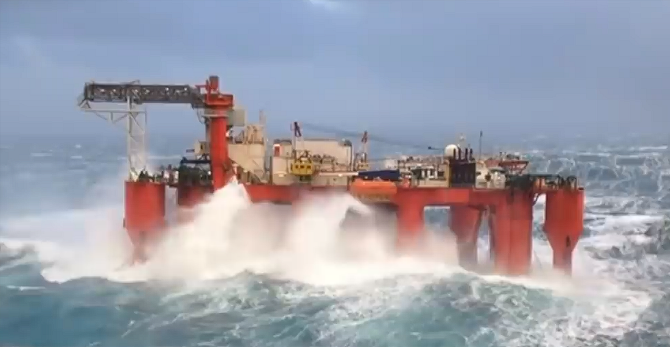
\includegraphics[height = 3cm]{figures/ch1-平台底部砰击.png}
		\caption{平台底部遭受波浪砰击}
    \label{fig:ch1-平台底部砰击}		
	\end{subfigure}
	\begin{subfigure}[b]{0.4\textwidth}
		\centering
		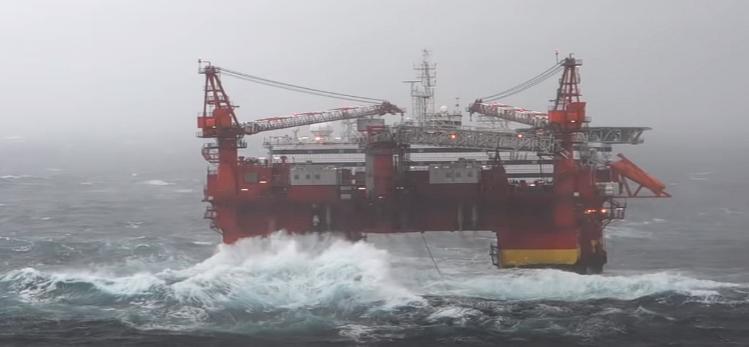
\includegraphics[height = 3cm]{figures/ch1-平台立柱砰击.png}
		\caption{平台立柱遭受波浪砰击}
    \label{fig:ch1-平台立柱砰击}
	\end{subfigure}
	\caption{北海石油钻井平台遭受波浪砰击(图片来自网络)}
	\label{fig:ch1-北油平台砰击}
\end{myfigure}

浮式平台所遭受的波浪砰击、上浪等强非线性作用会对平台造成严重危害。%
波浪砰击会产生极大的强非线性瞬时砰击载荷，对平台结构的安全性能是巨大的考验；%
而平台上浪可能会对甲板上的设施设备甚至人员安全造成威胁，引发严重的安全事故。%
因此对这类强非线性波浪结构物相互作用的问题进行研究和分析是十分必要的。%
然而这一类强非线性波浪结构物相互作用的问题一般涉及液面喷溅、空气卷吸以及结构运动等现象，%
属于气液固耦合的复杂动力学问题，一直以来都是船舶与海洋工程中的研究重点和难点\cite{faltinsenSlammingMarineApplications2004}。%
针对该问题，学者们提出了各种理论分析、数值模拟和试验研究方法。%
其中理论分析由于假设的高度简化，一般只适用于一些简单结构以及线性或弱非线性波浪结构物相互作用问题；%
而模型试验耗费大、周期长、对试验技术与设备的要求高，具有较大的局限性。%
相反地，数值模拟耗费小、周期短、受环境影响小且可获得更为丰富的流场信息，%
尤其是计算流体动力学(Computational Fluid Dynamics，简称CFD)方法能够有效处理复杂强非线性波浪结构物相互作用问题，%
现已逐渐成为研究这类问题的重要手段\cite{zhouNumericalModellingDynamic2019,%
paulsenProbabilityWaveSlamming2019,%
zhuExperimentalInvestigationBreaking2022,%
huoStudyWaveSlamming2023}。%

浮式平台与固定式平台不同，在畸形波、风暴潮等恶劣海况下会产生大幅度运动，%
该运动同时也会影响波浪运动和平台受力，从而形成一个复杂的动态耦合系统，%
使得结构物的运动响应和波浪载荷的准确预报更加困难\cite{张HaiYangJieGouWuBoLangPengJiDeShuZhiYanJiuZongShu2023}，%
如\cref{fig:ch1-动态耦合系统}所示。%
因此在对浮式平台波浪砰击、上浪等问题进行强非线性载荷数值预报时，%
需要同时考虑大尺度极端波浪的生成、波浪的辐射和绕射，%
平台近场小尺度区域的瞬态砰击、上浪过程，以及平台在波浪中的载荷和运动响应。%
\begin{myfigure}
	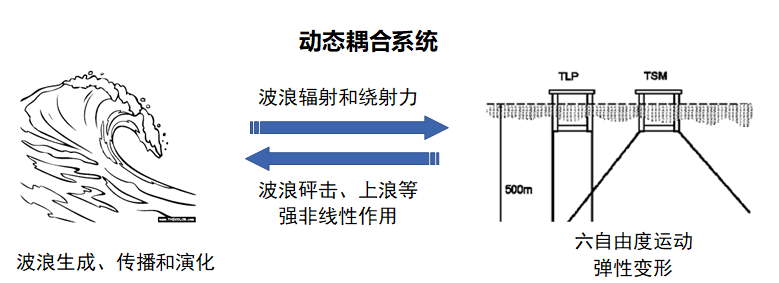
\includegraphics[width = 12cm]{figures/ch1-动态耦合系统.png}
	\caption{波浪-浮式平台动态耦合系统}
  \label{fig:ch1-动态耦合系统}
\end{myfigure}

\subsubsection{
  \texorpdfstring{数值方法需求} % 正文和目录中显示的标题
  {\thesubsubsection 数值方法需求} % 书签页中显示的标题
}
\label{sssec:数值方法需求}

对于波浪砰击、平台上浪这类局部存在大梯度流场和大变形自由液面的强非线性相互作用问题，%
采用VOF(Volume of Fluid)方法捕捉自由液面的有限体积法(Finite Volume Method，简称FVM)%
\cite{xieNumericalPredictionSlamming2018,bilandiNumericalSimulationVertical2018a}%
和无网格的光滑粒子流体动力学(Smoothed Particle Hydrodynamics，简称SPH)%
\cite{ogerTwodimensionalSPHSimulations2006a,%
shaoIncompressibleSPHSimulation2009,%
gaoNumericalModellingRegular2012a,%
sunSuctionEffectFreak2019}相对于其他数值方法更具有优势\cite{张HaiYangJieGouWuBoLangPengJiDeShuZhiYanJiuZongShu2023}。%

现有的强非线性波浪浮式平台相互作用数值研究主要集中于水槽/水池计算，%
多采用FVM方法进行流场离散，并通过VOF方法捕捉自由面。%
Liang等人\cite{liangNumericalStudyAir2010}%
通过VOF两相流求解器以及DNV船级社强度分析软件SESAM中的深水浮式系统锚泊耦合分析DeepC模块，%
对不规则波浪中处于系泊状态下的半潜式平台进行了波浪砰击的气隙响应研究。%
刘亚秋\cite{刘BanQianShiPingTaiDuoLiZhuBoLangPaShengYuPengJiTeXingYanJiu2019}%
使用CFD软件FINE/Marine对半潜式平台立柱的波浪爬升问题进行研究，%
主要分析了波浪参数对爬升现象的影响，并且研究了立柱参数对平台波浪爬升的影响。%
安康等人\cite{安TuoHangGongKuangXiaBanQianPingTaiChengGanDuiBoLangPengJiDeMinGanXing2020,%
施TuoHangGongKuangXiaBanQianShiPingTaiHengChengBoLangPengJiTeXingShiYanYanJiu2021}%
采用动网格法和VOF两相流求解器对拖航工况下半潜平台撑杆的砰击问题进行了研究，%
包括不同测点位置、不同流速和浪向角下的砰击特性等。%
Yao等人\cite{yaoExperimentalNumericalInvestigation2023a}通过StarCCM+中的VOF方法追踪自由面以及六自由度动态耦合%
(Dynamic Fluid Body Interaction，简称DFBI)模型定义系泊缆和平台的运动，对恶劣海况下的半潜式平台进行了数值模拟。%

近年来，基于无网格描述的CFD方法在模拟强非线性波浪结构物相互作用方面受到了广泛的关注。%
Rudman和Cleary等人\cite{rudmanRogueWaveImpact2009,rudmanRogueWaveImpact2013,rudmanInfluenceMooringSystem2016}%
采用基于无网格描述的SPH法对极端环境下半潜式平台的水动力特性进行了数值研究，%
先后探究了不同系泊系统的浮式平台在波浪砰击作用下的运动响应，%
以及波浪入射角与系泊缆预张力对张力腿平台(Tension Leg Platfomathrm，简称TLP)运动幅值和系泊缆最大张力及松弛度的影响。%
研究表明，与有网格CFD技术相比，SPH法可以更有效地处理波浪破碎、波浪与结构物的强非线性相互作用等问题。%
值得注意的是在他们的计算中，物理时间80秒，需要单核CPU运行300小时。%
Pan等人\cite{panApplicationSPHMethod2016a}采用SPH方法对溃坝下游立方柱的砰击力以及极端波浪作用下的浮式平台的运动进行了计算，%
波浪与浮体相互作用的数值模型及计算结果如\cref{fig:ch1-TPL-SPH模拟}所示。%
\begin{myfigure}
	\begin{subfigure}[b]{0.6\textwidth}
		\centering
		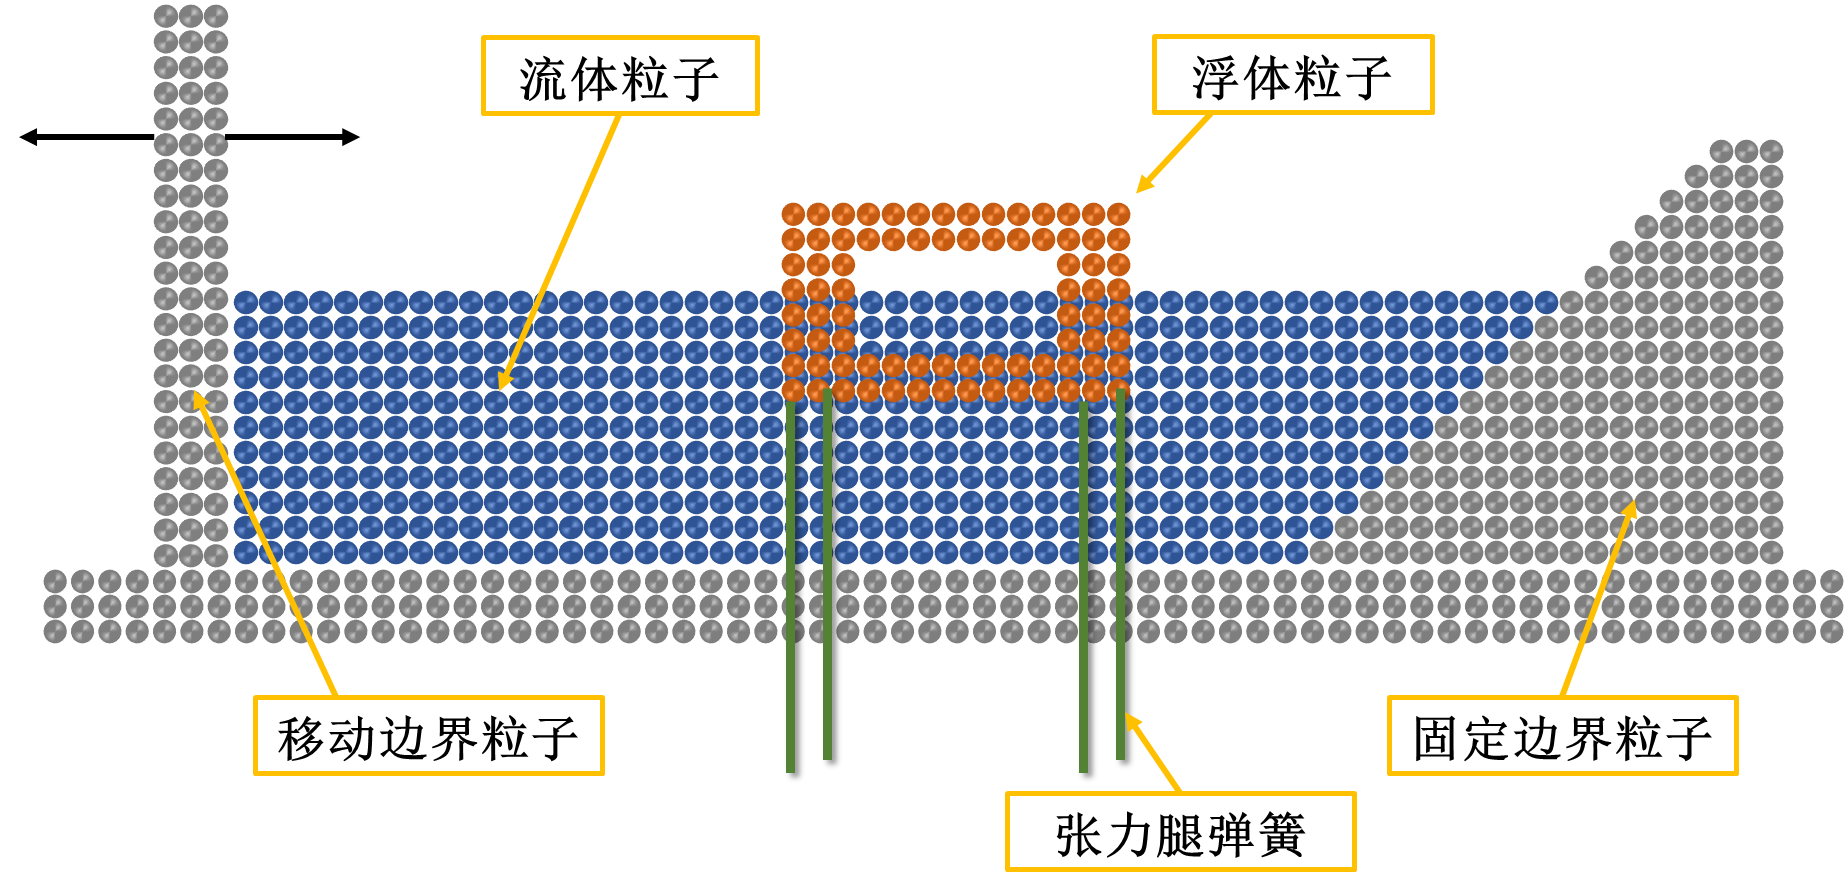
\includegraphics[width=\textwidth]{figures/ch1-TPL-SPH模型.png}
		\caption{极端波浪冲击平台的SPH数值模型}
    \label{fig:ch1-TPL-SPH模型}		
	\end{subfigure}
	\vspace*{3pt} % 调整竖直间隔
	\begin{subfigure}[b]{0.6\textwidth}
		\centering
		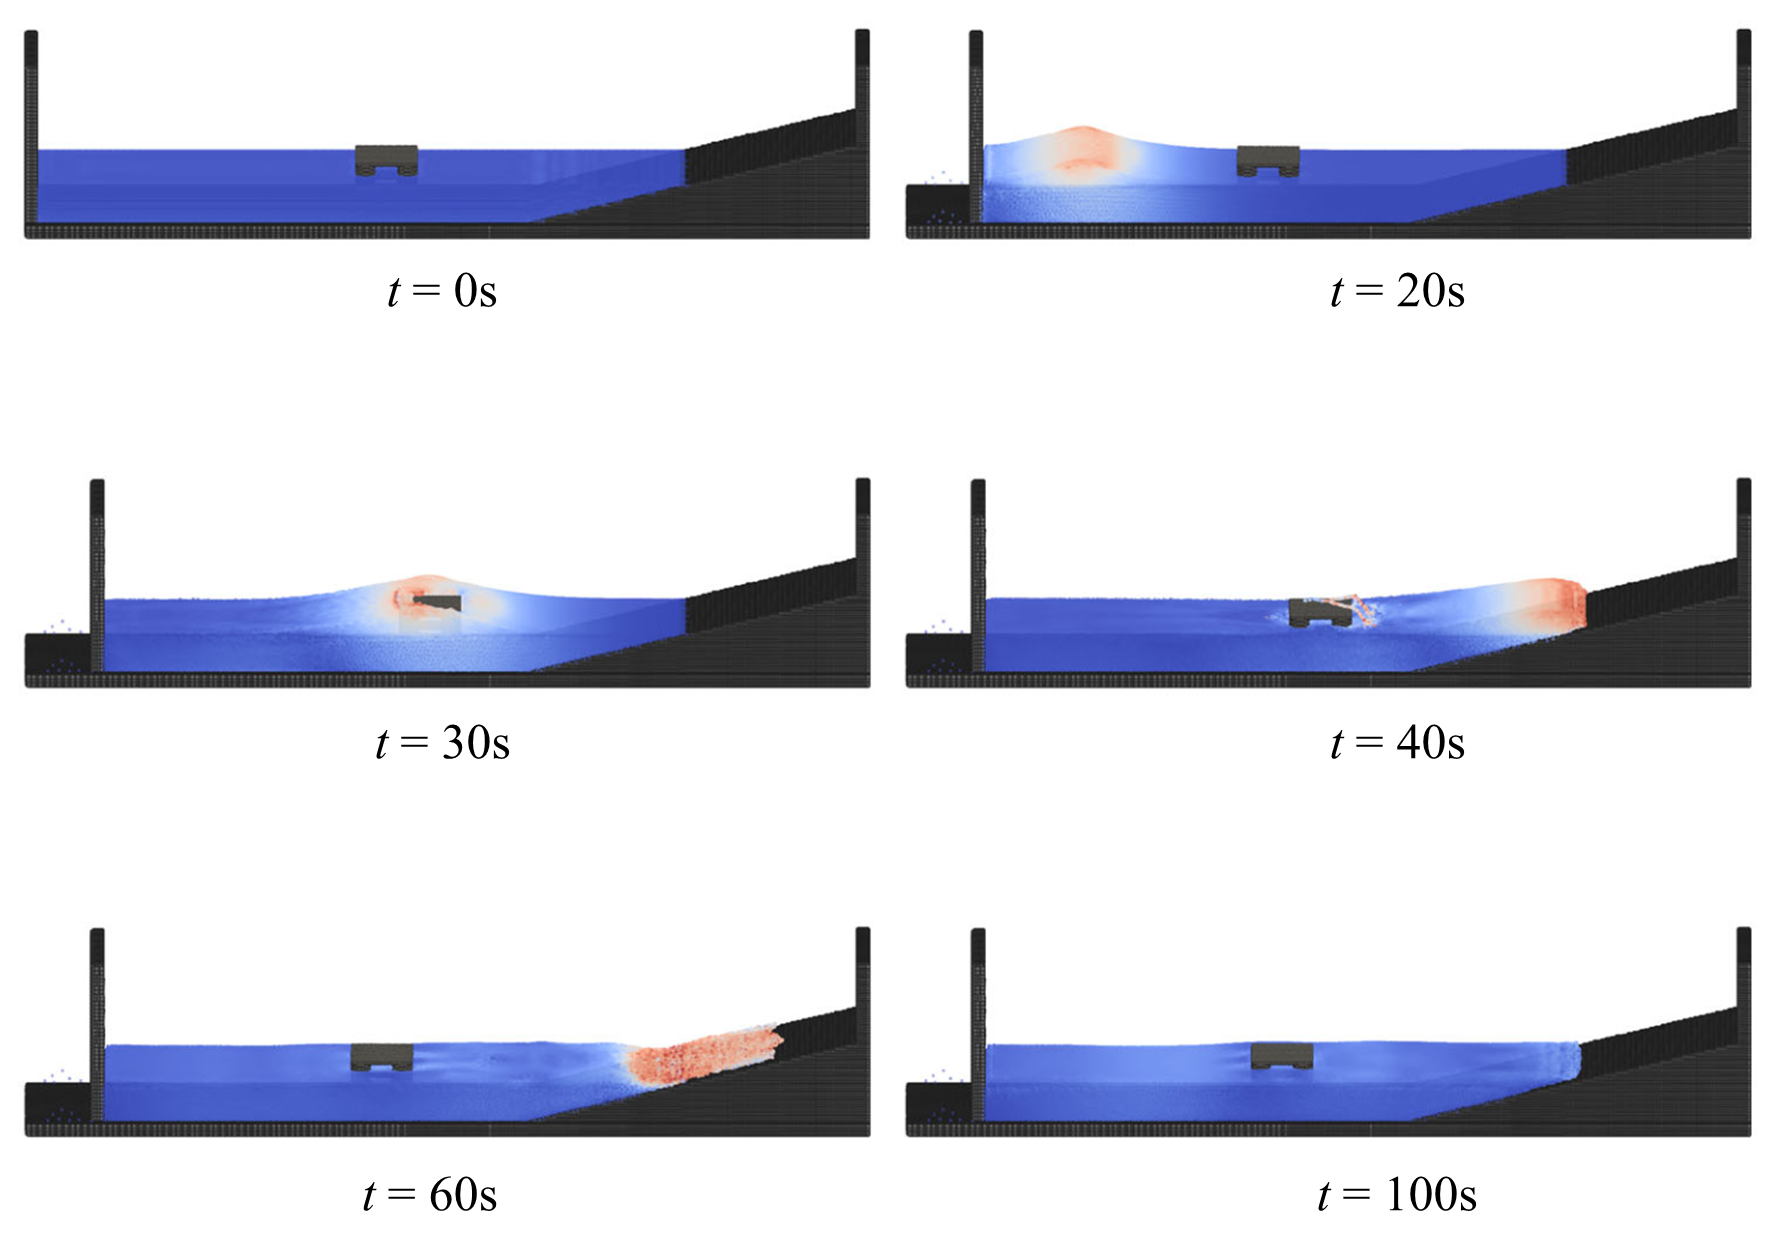
\includegraphics[width=\textwidth]{figures/ch1-TPL-结果.png}
		\caption{SPH模拟结果快照}
    \label{fig:ch1-TPL-结果}
	\end{subfigure}
	\caption{TLP波浪砰击的SPH方法数值计算模型及计算结果\cite{panApplicationSPHMethod2016a}}
	\label{fig:ch1-TPL-SPH模拟}
\end{myfigure}

数值结果和试验结果对比表明，SPH方法可以准确捕捉重力和惯性力驱动流中固定物体的复杂瞬态载荷特性以及浮式平台的刚体运动。%
此外他们对聚焦波下TLP的运动进行了数值模拟，并且将张力腿假设为弹簧模型，详细地分析了波浪冲击力以及张力腿所施加的反作用力。

研究人员对势流边界元方法和CFD方法在波浪浮式平台相互作用数值模拟方面进行了对比，%
发现势流方法的计算速度远远高于CFD方法，%
而CFD方法在受到粘性和强非线性因素影响较大的流场计算中更加准确。%
Rivera-Arreba等人\cite{rivera-arrebaModelingSemisubmersibleFloating2019}%
和Zhou等人\cite{zhouInvestigationFocusedWave2019}%
对比了势流方法和CFD方法在计算波浪中半潜式风机平台的运动响应和波浪力时的表现。%
其中，Rivera-Arreba等人\cite{rivera-arrebaModelingSemisubmersibleFloating2019}%
采用了基于势流理论的二阶边界元势流求解器和基于Navier-Stokes(NS)方程的VOF方法的两相流求解器，%
计算结果表明对于波陡不大的规则波，两种数值模拟方法均能很好地模拟结构物的响应；%
而对于大波陡波浪，由于势流求解器不能考虑粘性以及高阶非线性的影响，两种模型的计算结果存在差别。%
类似地，Zhou等人\cite{zhouInvestigationFocusedWave2019}在浮式风机平台的水动力计算中，%
通过对一阶、二阶势流结果以及CFD结果的对比分析，发现势流计算和CFD计算在靠近结构自然频率时的结果有很大的差别。%
在他们的工作中CFD部分的网格数量为235.4万，在360核CPU并行运算下，80小时能够完成200秒物理时间的模拟，%
而势流软件只需要40秒便可完成相应的物理计算。%

对于复杂构型浮式平台的波浪砰击、上浪等问题，采用VOF方法的FVM方法和SPH方法是现在普遍采用的数值手段。%
SPH方法相较于FVM方法得益于其拉格朗日和无网格粒子特性，对于自由液面或流固界面可自动完成追踪，并且精确满足质量守恒，%
因此比较适合于模拟强非线性作用过程中的液体喷溅和结构大幅运动等自由液面大变形和动边界过程。%
但是由于CFD方法的计算成本限制，对强非线性波浪浮式平台相互作用问题的数值模拟远远达不到工程需要。%

总的来说，在对波浪与浮式平台的强非线性作用进行数值预报时，%
需要同时考虑大尺度极端波浪的生成和演化、波浪的辐射和绕射，%
平台近场小尺度区域强非线性过程以及平台在波浪中的运动响应。%
基于势流理论的传统水动力分析方法难以准确计算强非线性流固耦合问题，%
而CFD方法由于计算量大且格式耗散性强等原因无法长时间准确捕捉波浪运动。%
因此，根据势流方法和CFD方法的特点，结合两者优势的势粘流耦合方法逐渐被关注。%
自上世纪八十年代以来，不少学者对势粘流耦合方法进行了探索和研究，%
然而对于耦合区域或耦合界面的处理尚存在诸多难点，%
同时对于实际工程中出现的开放海域砰击问题的研究依然处于起步阶段\cite{choiGrid2GridHOSWrapper2017}，%
因此建立一种能够模拟强非线性波浪浮体相互作用问题的高效求解器是十分必要的。%

综上，本文旨在面向海洋工程中的浮式平台遭受波浪强非线性作用这一问题背景，%
对势粘流耦合方法展开初步研究，以探索能够实现精细高效模拟波浪与浮式平台强非线性相互作用的可行方法，%
从而为后续工程应用中海上浮式平台的安全性评估和结构优化设计提供数值方法支撑。%

\subsection{
  \texorpdfstring{势粘流耦合方法研究现状} % 正文和目录中显示的标题
  {\thesubsection 势粘流耦合方法研究现状} % 书签页中显示的标题
}
\label{ssec:势粘流耦合方法研究现状}

数值模拟作为波浪与结构物相互作用研究的一种重要手段，被广泛应用于船舶与海洋工程水动力研究中。%
本文重点关注非线性波浪的生成和演化以及波浪与结构物相互作用两类问题的数值模拟方法。%
在数值模拟中，首先需要考虑非线性波浪的生成、长时间大尺度的传播演化，%
以及在波浪演化或与结构物作用过程中小尺度范围内可能发生的波浪破碎、空气卷吸等现象。%
此外，对于波浪与结构物相互作用问题，还需要考虑结构物壁面附近的流体粘性效应和有旋流动。%
要准确地对波浪与结构物相互作用问题进行模拟，需要考虑多尺度流动、非线性波浪、水气两相流以及粘性旋度等因素。%

在粘性、旋度等因素可忽略时，波浪的生成和演化以及波浪与结构物的相互作用问题可以通过势流理论进行求解。%
边界元方法\cite{hessCalculationNonliftingPotential1964,贺JianDanGreenHanShuFaQiuJieSanWeiShuiDongLiXiShu1986}、%
水弹性理论\cite{priceHydroelasticityMarineStructures1985,田ChuanBoShuiDanXingLiXueLiLunDeYanJiuJinZhan2008}%
等都基于势流理论对波浪中船舶和海上平台的动力响应进行分析，%
并且许多势流模型已经发展出了非线性理论，能够处理弱非线性\cite{袁ShenHaiFuShiJieGouWuXiBoXiTongDeFeiXianXingShiYuFenXi2011}%
甚至完全非线性\cite{sunTwoDimensionalFully2012a}问题。%
理论上，在无粘无旋且不可压缩流体假设下，势流理论的控制方程由NS方程简化为Laplace方程。%
通过半解析的势流方法进行求解时，问题在空间维度上被降阶因此能极大减小计算量，且对于开放域问题具有优势。%
同时由于势流模型的数值耗散低，在对大尺度波浪的生成和演化这一类问题进行模拟时计算精度和效率都较高。%
但是由于对流动进行了高度简化，势流理论无法解决复杂问题，如船舶的粘性阻力、涡激力、结构物周围的流动分离以及波浪破碎等。%

CFD方法，主要通过求解NS方程来模拟波浪与结构物相互作用的问题。%
CFD方法能够在模拟过程中考虑粘性、旋度以及湍流等，%
并且通过一些自由面捕捉方法如水平集方法\cite{sussmanLevelSetApproach1994} (Level Set Method，简称LSM)、%
VOF\cite{hirtVolumeFluidVOF1981} (Volume of Fluid，简称VOF)等可实现对两相流的模拟，%
因此采用CFD方法模拟波浪与结构物相互作用问题，%
能够更加精确地反映流动细节和结构物响应\cite{tezdoganFullscaleUnsteadyRANS2015,oggianoReproductionSteepLong2017,songValidationCFDApproach2020}。%
相应地，CFD方法相较于势流模型对计算资源的需求更大，当问题涉及的时空尺度较大且对精度要求较高时更是如此。%
同时，CFD方法的数值耗散较大，不适合进行长时间、大尺度波浪问题的模拟。%

Ransley等人\cite{ransleyBlindComparativeStudy2019,ransleyBlindComparativeStudy2020}%
的盲测中比较了几种CFD求解器和势流求解器对无破碎波浪与结构物相互作用问题的计算结果。%
在中等波陡波浪条件下，即使是最快的CFD求解器也比势流求解器慢1.5个数量级。%
但作者同时提出，如果势流理论的假设不再成立，即当波陡增大至波浪发生破碎时，只有使用CFD求解器才能很好地解决问题。%

船舶与海洋工程水动力研究中所涉及的流动问题一般为高雷诺数流动，流体的粘性主要作用于结构物面附近的薄层—即边界层内部，%
而边界层外部的流动由于能量耗散，其旋度和粘性影响在远离近场时会逐渐减小直至消失，可近似为无旋理想流动。%
因此在靠近结构物的内域采用CFD方法求解，而在远离结构物的外域采用势流方法求解，%
从而通过不同的模型来更高效地模拟不同的物理现象是十分自然的想法。%
在过去的几十年间有诸多学者对势粘流耦合进行了探索和研究，发展了许多不同的模型和方法，并且已将这些方法应用到各类问题中。%
下文将简述这两类势粘流耦合方法。%

\subsubsection{
  \texorpdfstring{区域分解方法} % 正文和目录中显示的标题
  {\thesubsubsection 区域分解方法} % 书签页中显示的标题
}
\label{sssec:区域分解方法}

区域分解方法是最早被用于进行势粘流耦合研究的方法。%
自二十世纪初Prandtl\cite{prandtlUberFlussigkeitsbewegungBei1904}提出边界层理论以来，学者们对粘流和无粘流间的耦合展开了诸多研究。%
在边界层理论中，流体的粘性效应主要体现在边界层内部，而在边界层外部流动可近似视为无粘流或理想流动。%
与边界层理论类似，区域分解方法的基本思路是将流域划分为势流域$\Omega_{\rm{PF}}$和粘流域$\Omega_{\rm{NS}}$，在不同流域采用不同的模型进行求解，并%
在耦合区域$\Omega_{\rm{Coupling Domain}}$或耦合界面$\Gamma_{\rm{Coupling}}$处进行耦合计算，%
以实现势流与粘流的耦合过程，如\cref{fig:ch1-DD-示意图}所示。
\begin{myfigure}
	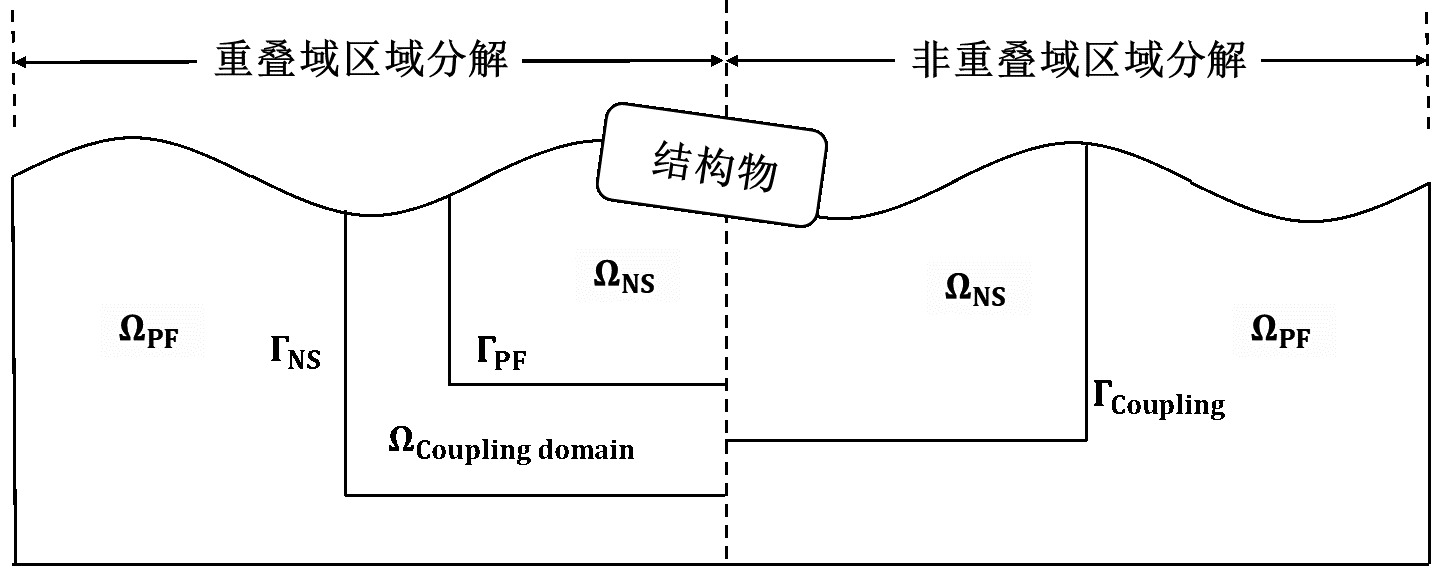
\includegraphics[width = 12cm]{figures/ch1-DD-示意图.png}
	\caption{区域分解方法示意图}
	\label{fig:ch1-DD-示意图}
\end{myfigure}

区域分解方法的关键在于势粘流模型、耦合方法和流域划分这三个方面，下文将对此展开介绍。%

(1)	势粘流模型%

势流理论是基于不可压、无粘、无旋假设建立的，其流动可以通过速度势描述，控制方程为Laplace方程；%
粘流方法的基本控制方程为连续性方程和NS方程，能够考虑流体的可压缩性和粘性效应。%

\cref{tab:ch1-DD-PFNS-models}中列举了一些以往区域分解方法研究中所采用的势粘流模型。%

\begin{mytable}
	\caption{区域分解方法中的势粘流模型}
	\label{tab:ch1-DD-PFNS-models}
	\begin{tabularx}{\textwidth}{c|c|X}
		\toprule
		{势粘流模型} & \multicolumn{2}{c}{方法类型} \\
		\midrule
		\multirow{11}{*}{势流模型} & \multirow{2}{*}{势流波浪模型} & {Boussinesq模型\cite{narayanaswamyHybridBoussinesqSPHWave2008,%
		christensenTransferBoussinesqWaves2009,kassiotisCouplingSPH1D2011,weiCostEffectiveMethodModelling2017}} \\
		& & {SWASH模型\cite{altomareCouplingSWASHSPH2014} (Simulating WAves till SHore model)} \\
		\cline{2-3}
		& \multirow{9}{*}{势流数值方法} & {边界元法\cite{campanaDomainDecompositionFree1994,campanaViscousinviscidCouplingFree1995,%
		guignardComputationShoalingBreaking1999,iafratiDomainDecompositionApproach2003,lachaumeModelingBreakingPostbreakingWaves2003,%
		biausserNumericalAnalysisInternal2004,drevardExperimentalValidationCoupled2005,colicchioBEMlevelSetDomaindecomposition2006,%
		kimSimpleTwowayCoupling2010,zhangCouplingViscousPotential2013,zhangSolitaryWaveBreaking2015,%
		孟JiYuShuangXiangShiLiuNianLiuOuHeDeShuZhiXiaoBoMoNi2022,sunWeakCouplingMPS2017,%
		taoApplicationAdvancedCoupled2022b} (Boundary Element Method，简称BEM)} \\
		& & {高阶谱法\cite{ogerCoupledSPHspectralMethod2014,nelliExperimentalNumericalModels2017,zhuangRegularIrregularWave2018,%
		choiGenerationRegularIrregular2018,韩ZhiLiYuanZhuBoLangPaShengHOSCFDShuZhiMoNi2019,%
		宋JiYuGaoJiePuFangFaYuCFDJiSuanDeOuHeMoXingZaiBuGuiZeBoMoNiZhongDeYingYong2019,%
		宋JiYuGaoJiePuFangFaYuCFDOuHeMoXingDeJiDuanBoLangShuZhiMoNi2019,庄GaoJiePuFangFaYuCFDFangFaOuHeDeShuZhiMoNiJiShu2019,%
		郭JiYuNianXingLiuHeNianShiLiuOuHeFangFaDeChuanBoBoLangZengZuYuYunDongXiangYingShuZhiYanJiu2020,%
		韩JiYuHOSCFDNianShiLiuOuHeFangFaMoNiZhiLiYuanZhuBoLangPaSheng2021,zhuangParametricStudyNew2021} (High Order Spectral，简称HOS)} \\
		& & {有限体积法\cite{kristiansenGapResonanceAnalyzed2012,luOverlappingDomainDecomposition2017} (Finite Volume Method，简称FVM)} \\
		& & {有限元法\cite{glowinskiDomainDecompositionMethods1983,dinhCouplingViscousInviscid1988,kimRingingAnalysisVertical2012,%
		baquetNumericalModelingUsing2017} (Finite Element Method，简称FEM)} \\
		& & {有限差分法\cite{paulsenEfficientDomainDecomposition2014,钟JiYuShiLiuNianLiuShuangXiangOuHeMoXingDeShuZhiZaoBo2022,%
		agarwalThreedimensionalCouplingBoussinesq2022} (Finite Difference Method，简称FDM)} \\
		& & {准拉格朗日欧拉有限元法\cite{liZonalHybridApproach2018,yanNumericalSimulationWave2019,zhang3DHybridModel2019,%
		zhang3DHybridModel2020,zhangNumericalStudyInteraction2021} (Quasi Lagrangian Eulerian Finite Element Method，简称QALE-FEM)} \\
		& & {无旋层析水波理论\cite{赵JiYuShiNianLiuDanXiangOuHeDeKCSBoLangZengZuYanJiu2018,%
		ZhaoShiNianLiuDanXiangOuHeDeZhiLiYuanZhuBoLangPaShengMoNi2019} (Irrotational Green-Naghdi，简称IGN)} \\
		& & {调和多项式单元法\cite{robauxAssessmentOnewayCoupling2022} (Hamathrmonic Polynomial Cell，简称HPC)} \\
		\hline
		\multirow{7}{*}{粘流模型} & \multirow{2}{*}{有网格方法} & {FVM\cite{narayanaswamyHybridBoussinesqSPHWave2008,%
		campanaViscousinviscidCouplingFree1995,guignardComputationShoalingBreaking1999,iafratiDomainDecompositionApproach2003,%
		lachaumeModelingBreakingPostbreakingWaves2003,biausserNumericalAnalysisInternal2004,drevardExperimentalValidationCoupled2005,%
		kimSimpleTwowayCoupling2010,孟JiYuShuangXiangShiLiuNianLiuOuHeDeShuZhiXiaoBoMoNi2022,nelliExperimentalNumericalModels2017,%
		zhuangRegularIrregularWave2018,choiGenerationRegularIrregular2018,韩ZhiLiYuanZhuBoLangPaShengHOSCFDShuZhiMoNi2019,%
		宋JiYuGaoJiePuFangFaYuCFDJiSuanDeOuHeMoXingZaiBuGuiZeBoMoNiZhongDeYingYong2019,庄GaoJiePuFangFaYuCFDFangFaOuHeDeShuZhiMoNiJiShu2019,%
		郭JiYuNianXingLiuHeNianShiLiuOuHeFangFaDeChuanBoBoLangZengZuYuYunDongXiangYingShuZhiYanJiu2020,%
		韩JiYuHOSCFDNianShiLiuOuHeFangFaMoNiZhiLiYuanZhuBoLangPaSheng2021,zhuangParametricStudyNew2021,kristiansenGapResonanceAnalyzed2012,%
		luOverlappingDomainDecomposition2017,glowinskiDomainDecompositionMethods1983,kimRingingAnalysisVertical2012,%
		paulsenEfficientDomainDecomposition2014,钟JiYuShiLiuNianLiuShuangXiangOuHeMoXingDeShuZhiZaoBo2022,liZonalHybridApproach2018,%
		赵JiYuShiNianLiuDanXiangOuHeDeKCSBoLangZengZuYanJiu2018,ZhaoShiNianLiuDanXiangOuHeDeZhiLiYuanZhuBoLangPaShengMoNi2019,%
		robauxAssessmentOnewayCoupling2022,hildebrandtSimulationFocusingWaves2013,liNumericalSimulationFocusing2018,%
		junxianModellingFocusedWave2020}} \\
		& & {FEM\cite{zhangCouplingViscousPotential2013,zhangSolitaryWaveBreaking2015,glowinskiDomainDecompositionMethods1983,%
		dinhCouplingViscousInviscid1988,hamiltonViscousinviscidMatchingWave2002}} \\
		\cline{2-3}
		& \multirow{5}{*}{无网格方法} & {光滑粒子流体动力学方法\cite{kassiotisCouplingSPH1D2011,altomareCouplingSWASHSPH2014,%
		weiCostEffectiveMethodModelling2017,taoApplicationAdvancedCoupled2022b,ogerCoupledSPHspectralMethod2014,%
		zhang3DHybridModel2019,zhang3DHybridModel2020,zhangNumericalStudyInteraction2021} (Smoothed Particle Hydrodynamics，简称SPH)} \\
		& & {移动粒子半隐式方法\cite{sunWeakCouplingMPS2017} (Moving Particle Semi-implicit，简称MPS)} \\
		& & {Rankine源无网格Petrov-Galerkin法\cite{agarwalThreedimensionalCouplingBoussinesq2022,sriramHybridMethodModelling2014,%
		kumarHybridNumericalModel2020} (Meshless Local Petrov-Galerkin method with Rankine Source，简称MPLG\_R)} \\
		\bottomrule
	\end{tabularx}
\end{mytable}

常用的势流模型主要为BEM和HOS方法。%
BEM作为一种半解析方法，能够将体网格计算转化为面网格计算，因此求解精度和计算效率都较高，并且适合处理开放边界问题。%
HOS方法作为一种伪谱法，在数值计算中引入了快速傅里叶变换，因此计算效率高且数值耗散低，适合长时间大尺度的波浪演算。%
粘流模型常用FVM方法离散流域，该方法守恒性好，网格对复杂几何区域的适应性强，并可通过VOF模型追踪自由面实现两相流的求解。%
SPH作为一种无网格方法，得益于其拉格朗日和无网格粒子特性，%
采用合适的离散格式即可实现自动捕捉自由液面\cite{colagrossiTheoreticalConsiderationsFreesurface2009}，%
并且精确满足质量守恒，因而在砰击、上浪等强非线性自由面问题的势粘流耦合中也被广泛应用。%

(2) 耦合方法%

耦合方法是区域分解方法的研究重点。%
从势粘流域是否重叠考虑，有重叠域耦合和非重叠域(即界面)耦合；%
从耦合方向考虑，可以分为单向耦合和双向耦合，即势粘流域间的信息是单向传递还是双向传递，也称为弱耦合和强耦合；%
从匹配方式考虑，主要有迭代匹配和松弛函数两种方法；%
从匹配的边界条件考虑，更是丰富多样，例如速度势Dirichlet条件，速度法向分量Neumann条件等。%
值得注意的是，对于船舶与海洋工程中的水动力问题，由于自由面的存在，不同区域匹配时所用的边界条件是耦合准确性和稳定性的关键。%

最早区域分解方法被用于空气动力学的势粘流耦合研究。%
Dinh等人\cite{glowinskiDomainDecompositionMethods1983,dinhCouplingViscousInviscid1988}针对不可压粘性流问题，%
按照距离物面远近将流域分为外部势流域和内部粘流域，并在两者间保留有重叠区域。%
粘流域提供速度势作为势流域的Dirichlet边界条件，势流域为粘流域提供速度边界条件，子域间迭代运算至收敛，%
收敛条件为重叠域内的势流速度势梯度和粘流速度满足最小二乘优化条件。%
在二维机翼绕流问题的计算中，通过FEM对势粘流控制方程进行离散，耦合方法的粘流域节点和单元数量相较于全粘流方法减少近1/3，%
并且计算给出的机翼表面压力分布、流线图和涡量场也与后者吻合良好。%
不过由于收敛所需的迭代计算量并不小，因此对计算效率的提高并不明显。%

Campana等人\cite{campanaDomainDecompositionFree1994,campanaViscousinviscidCouplingFree1995}%
将势粘流耦合方法引入至船舶水动力性能预报的研究中。%
与Dinh等人\cite{dinhCouplingViscousInviscid1988}的方法不同，%
Campana等人\cite{campanaDomainDecompositionFree1994}尝试取消势粘流重叠区域，仅通过界面进行耦合。%
在界面处，粘流域提供速度法向分量作为势流域的Neumann边界条件，而势流域提供速度和压力作为粘流域边界条件。%
对定常流中几类船型的计算结果显示，尽管能够收敛，但收敛速度不是很理想，并且在界面上观察到了非平滑过渡。%
因此Campana等人\cite{campanaViscousinviscidCouplingFree1995}将界面改为重叠区域，%
势流域在粘流边界Гp仅提供速度作为边界条件，而粘流域在势流边界Гv提供边界条件不变，如下：%
\begin{equation}
	\left.\bm{u}\right|_{\Gamma_{\rm{v}}} = \nabla\left.\phi\right|_{\Gamma_{\rm{v}}}, \qquad
	\left.\left(\frac{\partial \phi}{\partial n}\right)\right|_{\Gamma_{\rm{p}}} = \bm{u}\cdot\left.\bm{n}\right|_{\Gamma_{\rm{p}}}
\end{equation}
式中：$\phi$为速度势，$\bm{u}$为速度，$\bm{n}$为边界法向。%
采用该方法对几类船型进行模拟计算，给出的压力云图与全粘流方法和试验数据对照都吻合较好，而计算时间仅为全粘流方法的1/6。%
新方法提高了收敛速度，并保证了匹配面上的平滑过渡，但艏艉处的计算结果较差，试验中观察到的速度场S形轮廓并未出现。%

进一步地，Iafrati和Campana\cite{iafratiDomainDecompositionApproach2003}针对界面耦合提出了新的耦合边界条件，%
并与Campana\cite{campanaViscousinviscidCouplingFree1995}的重叠域耦合方法进行了对比。%
势流域提供速度和压力边界条件，粘流域通过非稳态Bernoulli方程获得界面上的速度势，为势流域提供Dirichlet边界条件，在界面Г上的边界条件如下：%
\begin{equation}
	\bm{u}_{\rm{v}} = \nabla \phi,\quad 
	p_{\rm{v}} = p_{\rm{p}} - 2\mu \frac{\partial \bm{u}_n}{\partial n}, \quad
	\phi = \int_{0}^{t}\frac{\partial \phi}{\partial t} {\rm{d}} t 
	= \int_{0}^{t} \left(-\frac{p_{\rm{v}}}{\rho} - \bm{g} - \frac{\left|\bm{u}_{\rm{p}}\right|^2}{2}\right) {\rm{d}} t 
\end{equation}
式中：$\phi$为速度势，$\bm{u}_{\rm{p}}$、$\bm{u}_{\rm{v}}$、$p_{\rm{p}}$和$p_{\rm{v}}$分别为势粘流域的速度及压力，%
$\bm{n}$为边界法向，$\rho$为流体密度。新的界面耦合方法相较于重叠域耦合，收敛速度更快，但误差略大。%
采用该方法对浸没水翼产生的破碎波进行模拟，能够将粘流域大小缩小至计算域的30\%。%
Zhang等人\cite{zhangCouplingViscousPotential2013,zhangSolitaryWaveBreaking2015}%
在Iafrati等人\cite{iafratiDomainDecompositionApproach2003}的基础上提出了新的隐式迭代方法，%
并加入了自由面校正和不匹配网格插值，模拟的溃坝过程与试验吻合较为一致。

Hamilton等人\cite{hamiltonViscousinviscidMatchingWave2002}将外域无粘自由表面流在圆柱界面上的广义解用“壳函数”(Shell Functions)表达，%
使界面上的速度和压力通过“壳系数”(Shell Coefficients)相关联。%
并且提出了一种新的“压力驱动”耦合方法，内域依赖外域在界面上提供压力以进行下一步计算。%
预求解并存储“壳系数”后，内域只需要提供界面处的速度，就能够通过“壳函数”获得外域在界面上的压力，达到一次求解、多次使用，从而实现更高效的界面耦合。%
对规则波圆柱绕流的模拟结果显示，耦合方法较势流方法计算的波浪力较小。%
除了依靠显式传递边界条件实现势粘流耦合，Kristiansen等人\cite{kristiansenGapResonanceAnalyzed2012}在势粘流域均采用FVM数值方法，%
并将粘流求解过程分解，从而能够在整场流域得到一个单一的方程组，隐式包含了势粘流域边界条件的交互。

孟巍等人\cite{孟JiYuShuangXiangShiLiuNianLiuOuHeDeShuZhiXiaoBoMoNi2022}结合松弛函数\cite{paulsenEfficientDomainDecomposition2014}%
和边界条件传递\cite{campanaDomainDecompositionFree1994}以实现双向耦合，%
即势流域向粘流域通过松弛函数传递波高和速度，而粘流域为势流域提供Neumann边界条件。%
通过该耦合方法实现的数值消波能够将粘流消波区减小为全粘流的1/5。%
钟文杰等人\cite{钟JiYuShiLiuNianLiuShuangXiangOuHeMoXingDeShuZhiZaoBo2022}采用了类似的方法，%
但松弛函数被用于粘流域向势流域传递波高和速度，而势流域在粘流域边界插值提供波高和速度条件。%
通过该方法实现的数值造波，能够在波浪传播接近粘流域入口时才开始粘流计算，进而节省计算时间。

上述耦合方法主要被用于波浪模型或势流数值方法等与有网格CFD方法间的耦合，%
而关于无网格CFD如光滑粒子流体动力学(Smoothed Particle Hydrodynamics，SPH)的耦合方法也有一定的发展。%
Narayanaswamy\cite{narayanaswamyHybridBoussinesqSPHWave2008}采用%
类似重叠区域耦合\cite{campanaViscousinviscidCouplingFree1995}的方式%
实现了Boussinesq波浪模型和SPH方法的耦合，对孤立波传播的模拟效果较好。%
Altomare等人\cite{altomareCouplingSWASHSPH2014}设置了一组速度由SWASH模型提供的SPH粒子，%
其形状在每一时间步变化，起到“造波桨”(Wave Paddle)的作用。%
通过这组“造波桨”粒子与自由流体粒子相作用而产生波浪，将势流域信息传递至粘流域中，实现了SWASH模型与SPH方法的单向耦合。%
该方法对规则波近岸浅化的模拟与试验结果对比一致性较好。%
Oger等人\cite{ogerCoupledSPHspectralMethod2014}在每一时间步，使用HOS方法将速度和压力赋给势粘流重叠域内的粒子，%
随后这些“受迫粒子”与粘流域内的“自由粒子”共同参与SPH计算以实现耦合。%
这里与Altomare等人\cite{altomareCouplingSWASHSPH2014}的方法不同，重叠域内的粒子会流入流出该区域，而非是固定的一组粒子，%
因此可以直接模拟波浪中水体的流动，而非通过造波桨\cite{altomareCouplingSWASHSPH2014}的移动产生波浪。

根据上述研究可知，耦合方法可以大致分为三类，\cref{tab:ch1-DD-models-characters}中简单总结了这几类常用耦合方法的部分特点。%
而边界条件的选取、耦合方向等方法细节在不同的研究中都有所不同，%
并且对于无网格粒子法有特殊的耦合方法，这些都要视具体问题而定。%
总而言之，耦合方法的关键在于精确地在势粘流域间传递流场信息(如速度、压力和波高等)，%
并且尽可能保证过渡区的平滑，解决在边界处可能出现的反射和发散等问题。
\begin{mytable}
	\caption{几类常用区域耦合方法的特点}
	\label{tab:ch1-DD-models-characters}
	\begin{tabularx}{\textwidth}{M{3.1cm} X X}
		\toprule
		{耦合方法} & {\centering 简介} & {\centering 特点} \\
		\midrule
		{重叠域迭代匹配} & {势粘流域互相在重叠域边界上提供边界条件，迭代计算至收敛} %
		& {势粘流域间过渡平滑，耦合精度较高；收敛速度较慢，计算效率提高不大} \\
		{界面迭代匹配} & {势粘流域在交界面处提供边界条件，迭代计算至收敛} %
		& {收敛速度较快，计算效率提高较大；势粘流域间过渡有间断，耦合精度略低}\\
		{重叠域松弛函数} & {通过重叠区域和松弛函数实现流场信息的传递} %
		& {无需迭代计算，对计算效率提高较大，松弛函数避免了反射波；非物理的耦合方法} \\
		\bottomrule
	\end{tabularx}
\end{mytable}

(3) 流域划分

在区域分解方法中，流域划分主要涉及势粘流域边界划分、势粘流域是否重叠、耦合区域的大小和位置或耦合界面的位置这几个问题，%
其中重叠区域在耦合方法中已经介绍，不在此赘述。其中，势粘流域边界划分将影响进出口边界、自由液面、物面等边界条件的处理。%

文献中对于流固耦合问题一般采用类似Campana等人\cite{campanaDomainDecompositionFree1994}的处理，%
将流域划分为结构物近场的粘流域和远场的势流域，自由面在势粘流域中都有分布。%
与之不同的是将自由面只包含于势流域或粘流域，例如Iafrati等人\cite{iafratiDomainDecompositionApproach2003}为了捕捉产生的波浪破碎现象，%
将流域上下划分，自由液面被完全包含于粘流域中，而浸没水翼在势流域中；%
Kristiansen等人\cite{kristiansenGapResonanceAnalyzed2012}将自由液面完全置于势流域内，%
仅将结构物底部发生流动分离的区域部分划为粘流域，因此他们的方法难以解决强非线性自由面问题。%

对于波浪生成和演化的流域划分，现有的研究主要关注强非线性自由面现象和数值波浪模拟两类。%
对于强非线性自由面问题，粘流域一般将强非线性现象发生的区域包含在内，%
如Guignard等\cite{guignardComputationShoalingBreaking1999}和%
Zhang等\cite{zhangCouplingViscousPotential2013,zhangSolitaryWaveBreaking2015}。%
对于数值波浪模拟问题，一般将势流域分布在粘流域的进出口以实现耦合造波或消波，%
如Baquet等\cite{baquetNumericalModelingUsing2017}和孟巍等\cite{孟JiYuShuangXiangShiLiuNianLiuOuHeDeShuZhiXiaoBoMoNi2022}。%

耦合区域的大小和位置或耦合界面的位置对于区域分解方法是一个较为复杂的问题，既要尽可能减小粘流域尺寸以提高计算效率，%
又需要保证粘流域的大小足以准确反映流动的粘性效应和强非线性现象等，并且需要考虑辐射波、绕射波的充分演化。%
Campana等人\cite{campanaViscousinviscidCouplingFree1995}对定常流中的S60船型进行模拟，%
耦合区域到船体的距离分别被设置为船长的1/20和1/100，其波高计算结果差距不大，这可能是由于该问题的非线性和粘性效应较弱。%
Iafrati等人\cite{iafratiDomainDecompositionApproach2003}对重叠域耦合的耦合区域宽度和界面耦合的界面位置都作了一定研究。%
当耦合区域的宽度较大时，不仅精度提高，收敛速度也有所增加。耦合界面的位置对速度结果影响较小，对波高几乎没有影响。%

Kim等人\cite{kimSimpleTwowayCoupling2010}针对BEM-FVM双向耦合方法，分析了耦合区域的宽度以及到结构物的距离对计算的影响。%
耦合区域宽度对波浪的计算结果影响并不大，并且除了波陡最小的一组试验，耦合方法的误差普遍小于全粘流方法。%
研究结论显示耦合区域到结构物的距离对一阶波幅影响不大，当距离为0.2和0.4倍波长时二阶波幅有较大差异，但当距离大于0.8倍波长时影响基本上消失。%
因此Kim等人\cite{kimSimpleTwowayCoupling2010}给出耦合区域到结构物的合适距离约为1.0倍波长。%
然而作者同时指出，流场中涡旋的强度可能由于波浪与结构物之间相互作用的强度而有所不同。因此对于不同问题，在选取该距离时还需要进一步的考虑。%

Zhuang等人\cite{zhuangParametricStudyNew2021}对基于松弛函数耦合的HOS-CFD单向耦合进行了较为丰富的参数化分析，%
其中也讨论了粘流域大小对计算的影响。通过对比三种大小的粘流域计算结果可以知道，当粘流域较小时船体周围的散射波无法充分演化，并且会出现更严重的反射波。%

区域分解方法通过将流域划分为不同子域，在子域内采用合适的模型进行求解，并通过重叠区域或界面实现子域间的信息匹配。%
因此对于区域分解方法来说，关键在于针对不同的问题和感兴趣的部分选择合适的耦合方法和势粘流模型。%
例如，对于波浪与结构物相互作用的问题，如果主要关心结构物的动力响应而忽略流场的细节，一般选择单向耦合。%
近几年研究者们倾向于采用松弛函数的耦合方法，而非通过迭代运算进行匹配耦合。%
这样做的好处是能够大幅减小计算量，避免了子域内重复的迭代运算，但是需要采取一定的手段以避免计算结果发散。%
此外，研究人员们对势粘流模型的选择十分多样，不同类型的问题需要选择合适的势粘流模型进行组合求解。

总的来说，基于区域分解的势粘流耦合方法经过一段时间的探索，已经在许多工程问题中得到了检验，\cref{tab:ch1-DD-progress}中列举了其中的一部分工作。%
在数值模拟中采用合适的耦合方法，能够在保证求解精度的前提下有效减少计算资源消耗，提高计算效率。%
现有的一些研究表明，在同等精度下耦合方法所耗计算时间能够减小至全粘流法的1/3%
\cite{赵JiYuShiNianLiuDanXiangOuHeDeKCSBoLangZengZuYanJiu2018}、%
1/6\cite{campanaViscousinviscidCouplingFree1995}甚至1/8\cite{robauxAssessmentOnewayCoupling2022}。%
波浪结构物相互作用的盲测试验系列\cite{ransleyBlindComparativeStudy2019,ransleyBlindComparativeStudy2020}中也采用了几类耦合方法，%
在计算效率上可以体现出相较于粘流方法的优势。%
不过耦合方法对计算效率的提高程度受许多方面的影响，如问题规模、非线性强度、耦合方式和并行策略等，还需进一步地探索。%
\begin{mylongtable}
	{M{3.0cm} M{1.15cm} M{1.15cm} M{2.0cm} M{1.6cm} M{1.2cm} M{5.2cm}} % 表格列宽设置
	{区域分解方法研究进展} % 题注
	{tab:ch1-DD-progress} % 标签
	{% 首页表头
		\toprule
		\multirow{2}{*}{代表性研究} & \multicolumn{2}{c}{边界条件} & {势流} & \multicolumn{2}{c}{粘流} & \multirow{2}{*}{应用问题} \\
		\cline{2-3} \cline{5-6}
		& \multicolumn{2}{c}{势流$\leftarrow\rightarrow$粘流} & {求解器} & \multicolumn{2}{c}{求解器/自由面技术} & \\
		\midrule}
	{% 后续页表头
		\multicolumn{7}{c}{\cref{tab:ch1-DD-progress} 区域分解方法研究进展(续表)} \\
		\toprule
		\multirow{2}{*}{代表性研究} & \multicolumn{2}{c}{边界条件} & {势流} & \multicolumn{2}{c}{粘流} & \multirow{2}{*}{应用问题} \\
		\cline{2-3} \cline{5-6}
		& \multicolumn{2}{c}{势流$\leftarrow\rightarrow$粘流} & {求解器} & \multicolumn{2}{c}{求解器/自由面技术} & \\
		\midrule}
	{\bottomrule} % 除最后一页外的表尾
	{\bottomrule} % 最后一页的表尾
	% 表格内容
	{Dinh等\cite{glowinskiDomainDecompositionMethods1983,dinhCouplingViscousInviscid1988} (1988)} %
	& {$\bm{u}$} & {$p$} & {FEM} & {FEM} & {——} & {机翼绕流 (2D)} \\
	{Campana等\cite{campanaDomainDecompositionFree1994} (1994)} %
	& {$\bm{u}_\tau, p$} & {$\phi_n$} & {BEM} & {FVM} & {——} & {定常流中几类船型的响应 (3D)} \\
	{Campana等\cite{campanaViscousinviscidCouplingFree1995} (1995)} %
	& {$\bm{u}$} & {$\phi_n$} & {BEM} & {FVM} & {——} & {定常流中几类船型的响应 (3D)} \\
	{Guignard等\cite{guignardComputationShoalingBreaking1999} (1999)} %
	& {$\bm{u}, p$} & {——} & {BEM} & {FVM} & {VOF} & {近岸波浪浅化、破碎 (2D)} \\
	{Iafrati等\cite{iafratiDomainDecompositionApproach2003} (2003)} %
	& {$\bm{u}, p$} & {$\phi$} & {BEM} & {FVM} & {——} & {浸没水翼产生破碎波 (2D)} \\
	{Lachaume\cite{lachaumeModelingBreakingPostbreakingWaves2003} (2003)} %
	& {$\bm{u}, p$} & {——} & {BEM} & {FVM} & {VOF} & {斜坡上孤立波的演化 (2D)} \\
	{Biausser\cite{biausserNumericalAnalysisInternal2004} (2004)} %
	& {$\bm{u}, p$} & {——} & {BEM} & {FVM} & {VOF} & {孤立波浅滩破碎 (2D、3D)} \\
	{Drevard等\cite{drevardExperimentalValidationCoupled2005} (2005)} %
	& {$\bm{u}, p$} & {——} & {BEM} & {FVM} & {VOF} & {孤立波跨越台阶破碎、浅滩破碎 (2D)} \\
	{Colicchio等\cite{drevardExperimentalValidationCoupled2005} (2005)} %
	& {$\bm{u}, p, \eta$} & {$\phi_n, p, \eta$} & {BEM} & {FDM} & {LSM} & {溃坝、甲板上浪 (2D)} \\
	{Narayanaswamy\cite{narayanaswamyHybridBoussinesqSPHWave2008} (2008)} %
	& {$\bm{u}$} & {$\bm{u}, \eta$} & {Boussinesq模型} & {SPH} & {——} & {孤立波恒定水深传播 (2D)} \\
	{Christensen等\cite{christensenTransferBoussinesqWaves2009} (2009)} %
	& {$\bm{u}, \eta$} & {——} & {Boussinesq模型} & {FVM} & {VOF} & {不规则波单桩载荷 (3D)} \\
	{Kim等\cite{kimSimpleTwowayCoupling2010} (2010)} %
	& {$\bm{u}, \eta$} & {$\phi_n, \eta$} & {BEM} & {FVM} & {VOF} & {规则波、随机波的传播 (2D)} \\
	\makecell{Hamilton等\cite{hamiltonViscousinviscidMatchingWave2002,hamiltonViscousInviscidMatching2011} \\(2002, 2011)} %
	& {$p$} & {$\bm{u}$} & {BEM} & {FEM} & {——} & {规则波传播、单桩载荷 (3D)} \\
	{Kassiotis等\cite{kassiotisCouplingSPH1D2011} (2011)} %
	& {$\bm{u}, \eta$} & {——} & {Boussinesq模型} & {SPH} & {——} & {规则波传播、与防波堤作用 (3D)} \\
	{Kim等\cite{kimRingingAnalysisVertical2012} (2012)} %
	& {$\bm{u}, \alpha$} & {——} & {FEM} & {FVM} & {VOF} & {不同波浪下单桩激振载荷 (3D)} \\
	{Kristiansen等\cite{kristiansenGapResonanceAnalyzed2012} (2012)} %
	& {$\phi$} & {$p$} & {FVM} & {FVM} & {——} & {双体结构强迫垂荡 (2D)} \\
	{Hildebrandt等\cite{hildebrandtSimulationFocusingWaves2013} (2013)} %
	& {$\bm{u}, p$} & {——} & {FEM} & {FVM} & {VOF} & {波浪冲击三角架结构 (3D)} \\
	{Paulsen等\cite{paulsenEfficientDomainDecomposition2014} (2014)} %
	& {$\bm{u}, \alpha$} & {——} & {FEM} & {FVM} & {VOF} & {不同波浪下竖直圆柱响应 (3D)} \\
	{Altomare等\cite{altomareCouplingSWASHSPH2014} (2014)} %
	& {$\bm{u}$} & {——} & {SWASH} & {SPH} & {——} & {近岸波浪浅化 (2D)} \\
	{Oger等\cite{ogerCoupledSPHspectralMethod2014} (2014)} %
	& {$\bm{u}, p$} & {——} & {HOS} & {SPH} & {——} & {FPSO模型甲板上浪 (3D)} \\
	{Sriram等\cite{sriramHybridMethodModelling2014} (2014)} %
	& {$\bm{u}, p$} & {$\phi$} & {FEM} & {IMLPG\_R} & {——} & {波浪传播、孤立波越过海堤 (2D)} \\
	\makecell{Zhang等\cite{zhangCouplingViscousPotential2013,zhangSolitaryWaveBreaking2015} \\(2013, 2015)} %
	& {$\bm{u}, p$} & {$\phi$} & {BEM} & {FEM} & {LSM} & {溃坝、孤立波传播和浅滩破碎 (2D、3D)} \\
	{Nelli等\cite{nelliExperimentalNumericalModels2017} (2017)} %
	& {$\eta$} & {——} & {HOS} & {FVM} & {VOF} & {波浪与系泊薄浮板作用 (3D)} \\
	{Lu等\cite{luOverlappingDomainDecomposition2017} (2017)} %
	& {$\bm{u}, \eta$} & {$\phi_n, \eta$} & {BEM} & {FVM} & {VOF} & {波浪浅化、浮式平台下沉 (2D、3D)} \\
	{Choi等\cite{choiGenerationRegularIrregular2018} (2018)} %
	& {$\bm{u}, \alpha$} & {——} & {HOS} & {FVM} & {VOF} & {规则波、不规则波、极端波浪生成 (2D、3D)} \\
	\makecell{赵彬彬等\cite{赵JiYuShiNianLiuDanXiangOuHeDeKCSBoLangZengZuYanJiu2018,%
	ZhaoShiNianLiuDanXiangOuHeDeZhiLiYuanZhuBoLangPaShengMoNi2019} \\(2017, 2018, 2019)} %
	& {$\bm{u}, \alpha$} & {——} & {IGN} & {FVM} & {VOF} & {KCS波浪增阻、直立圆柱波浪爬升 (3D)} \\
	{Li和Yan等\cite{liZonalHybridApproach2018,yanNumericalSimulationWave2019} (2018, 2019)} %
	& {$\bm{u}, p, \eta$} & {——} & {QALE-FEM} & {FVM} & {VOF} & {聚焦波与FPSO结构作用 (3D)} \\
	{Kumar等\cite{kumarHybridNumericalModel2020} (2020)} %
	& {$\bm{u}, p$} & {$\phi$} & {FEM} & {MLPG\_R} & {——} & {波浪爬升、近岸破碎 (2D)} \\
	{Wang等\cite{junxianModellingFocusedWave2020} (2020)} %
	& {$\bm{u}, p$} & {——} & {QALE-FEM} & {FVM} & {VOF} & {波浪与波浪能装置作用 (3D)} \\
	\makecell{Zhang等\cite{zhang3DHybridModel2019,zhang3DHybridModel2020,zhangNumericalStudyInteraction2021} \\(2019, 2020, 2021)} %
	& {$\bm{u}, p$} & {——} & {QALE-FEM} & {SPH} & {——} & {波浪与浮体、波浪能装置作用 (3D)} \\
	{宋家琦等\cite{宋JiYuGaoJiePuFangFaYuCFDJiSuanDeOuHeMoXingZaiBuGuiZeBoMoNiZhongDeYingYong2019,宋JiYuGaoJiePuFangFaYuCFDOuHeMoXingDeJiDuanBoLangShuZhiMoNi2019} (2019)} %
	& {$\bm{u}, \alpha$} & {——} & {HOS} & {FVM} & {VOF} & {规则波、不规则波、极端波浪生成 (2D、3D)} \\
	\makecell{庄园等\cite{zhuangRegularIrregularWave2018,庄GaoJiePuFangFaYuCFDFangFaOuHeDeShuZhiMoNiJiShu2019,%
	zhuangParametricStudyNew2021} \\(2018, 2019, 2021)} %
	& {$\bm{u}, \alpha$} & {——} & {HOS} & {FVM} & {VOF} & {KCS波浪增阻、波浪中FPSO船液舱晃荡 (2D、3D)} \\
	\makecell{韩勃等\cite{韩ZhiLiYuanZhuBoLangPaShengHOSCFDShuZhiMoNi2019,%
	韩JiYuHOSCFDNianShiLiuOuHeFangFaMoNiZhiLiYuanZhuBoLangPaSheng2021} %
	\\(2019, 2021)} %
	& {$\bm{u}, \alpha$} & {——} & {HOS} & {FVM} & {VOF} & {直立圆柱波浪爬升 (3D)} \\
	{孟巍等\cite{孟JiYuShuangXiangShiLiuNianLiuOuHeDeShuZhiXiaoBoMoNi2022} (2022)} %
	& {$\bm{u}, \eta$} & {$\bm{u}$} & {BEM} & {FVM} & {VOF} & {数值消波 (2D)} \\
	{钟文杰等\cite{钟JiYuShiLiuNianLiuShuangXiangOuHeMoXingDeShuZhiZaoBo2022} (2022)} %
	& {$\bm{u}, \eta$} & {$\phi, \eta$} & {FDM} & {FVM} & {VOF} & {数值造波 (2D)} \\
	{Robaux等\cite{robauxAssessmentOnewayCoupling2022} (2022)} %
	& {$\bm{u}, p$} & {——} & {HPC} & {FVM} & {VOF} & {波浪与固定潜体作用 (2D)} \\
	{Agarwal等\cite{agarwalThreedimensionalCouplingBoussinesq2022} (2022)} %
	& {$\bm{u}, p$} & {——} & {FEM} & {MLPG\_R} & {——} & {直立圆柱波浪爬升 (3D)} \\
	{Sriram等\cite{saincherThreeDimensionalHybrid2022} (2022)} %
	& {$\bm{u}, p$} & {——} & {FEM} & {FVM} & {VOF} & {固定/移动圆柱波浪爬升 (3D)} \\
	\makecell{郭浩等\cite{郭JiYuNianXingLiuHeNianShiLiuOuHeFangFaDeChuanBoBoLangZengZuYuYunDongXiangYingShuZhiYanJiu2020,%
	GuoJiYuNianShiLiuOuHeFangFaDeKCSChuanYunDongXiangYingYuBoLangZengZuShuZhiYanJiu2023} \\(2020, 2023)} %
	& {$\bm{u}, \alpha$} & {——} & {HOS} & {FVM} & {VOF} & {KCS波浪增阻 (3D)} \\
\end{mylongtable}

\subsubsection{
  \texorpdfstring{方程分解方法} % 正文和目录中显示的标题
  {\thesubsubsection 方程分解方法} % 书签页中显示的标题
}
\label{sssec:方程分解方法}

除了将流域在空间上划分为不同区域外，还有学者提出了对控制方程进行分解的方法。%
方程分解方法虽然是从流动控制方程中将势流部分解耦，但是其能够减小计算成本的原因还是由于粘性效应主要集中在物面附近，%
或者将势流部分去除入射波之后的流场波面只在结构物周围有比较大的波动，因此粘流模型仅在近场需要分布密网格，而在远场可以采用粗网格以减小计算消耗。%
方程分解方法主要有两种：一是基于Helmholtz速度分解的控制方程分解；%
二是基于SWENSE(Spectral Wave Explicit Navier-Stokes equations)模型的方程分解，%
下面将对其分别介绍。

Kim等人\cite{kimComplementaryRANSEquations2005}基于Helmholtz速度分解，%
如\cref{fig:ch1-Helmholtz-示意图}所示，将满足NS方程的整场速度分解为势流项$\bm{u}_{\rm{p}}$和粘流项$\bm{u}^*$：%
\begin{equation}
	\bm{u} = \bm{u}_{\rm{p}} + \bm{u}^*,\quad \bm{u} = \nabla \phi
\end{equation} 
将压力场进行同样的分解，进而推导出互补RANS方程：%
\begin{equation}
	\frac{\partial\bm{u}^*}{\partial t} + \left(\bm{u}^*\cdot\nabla\right)\bm{u}^* %
	+ \left(\bm{u}^*\cdot\nabla\right)\bm{u}_{\rm{p}} + \left(\bm{u}_{\rm{p}}\cdot\nabla\right)\bm{u}^* %
	= - \nabla p^* + \frac{\nabla^2\bm{u}^*}{\rm{Re}}
\end{equation}

式中Re为无量纲数雷诺数。在互补RANS方程中，粘流项在远场中快速耗散，因此可以在远场采用稀疏网格从而减少计算量。%
该耦合模型需要首先对势流部分求解，然后将势流项解代入互补RANS方程，进而求解获得粘流项解。%
Kim等人\cite{kimComplementaryRANSEquations2005}通过对空气动力学中的二维平板流、方形管道流动和机翼绕流进行数值模拟，%
并且与试验结果和传统RANSE求解器结果进行对比，验证了该方法有效性和准确性，二维平板流结果如\cref{fig:ch1-Helmholtz-Kim}所示。
\begin{myfigure}
	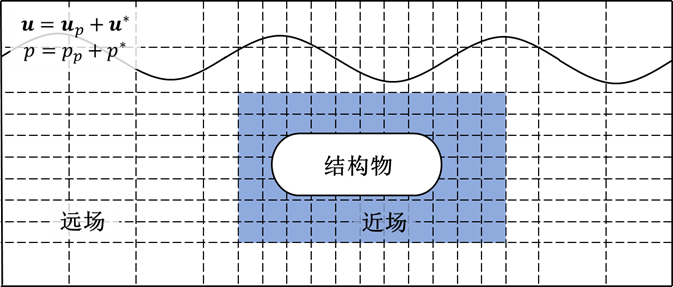
\includegraphics[width=0.6\textwidth]{figures/ch1-Helmholtz-示意图.png}
	\caption{Helmholtz速度分解示意图}
	\label{fig:ch1-Helmholtz-示意图}
\end{myfigure}
\begin{myfigure}
	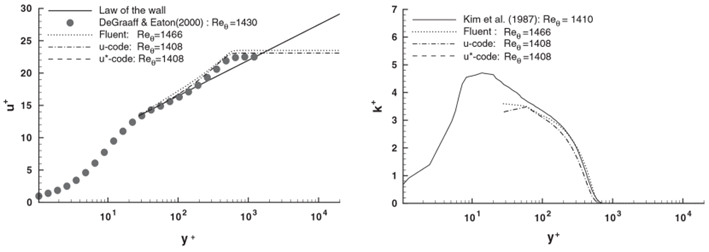
\includegraphics[width=0.9\textwidth]{figures/ch1-Helmholtz-Kim.png}
	\caption{二维平板流平均流向速度(左)和湍流动能(右)\cite{kimComplementaryRANSEquations2005}：耦合方法、全粘流方法和试验结果对比}
	\label{fig:ch1-Helmholtz-Kim}
\end{myfigure}

Hafez等人\cite{hafezImprovedNumericalSimulations2007}通过修正Bernoulli方程求得势流压力，并将其代入粘流方程求解。%
使用该方法分别对中等雷诺数不可压条件下，定常和非定常的二维翼型绕流进行了计算，结果与全粘流方法吻合较好。%
上海交通大学的赵骥、朱仁传等人\cite{ZhaoChuanBoShuiDongLiDeNianShiLiuOuHeFangFaChuTan2015,%
ZhaoJiYuHelmholtzSuDuFenJieDeNianShiLiuOuHeFangFa2016,%
ZhaoQiuJieSUBOFFRaoLiuWenTiDeNianShiLiuOuHeFangFa2017}使用该方法实现了二维圆柱绕流模拟，%
并在此基础上推广至三维，实现了三维潜体绕流的耦合计算。%
并且使用该方法计算了Wigley船的航行阻力，其中兴波阻力通过势流方法求解，而粘性阻力使用势粘流耦合方法求解获得，计算结果与试验和文献数据吻合较好。

Edmund等人\cite{edmundVelocityDecompositionMethod2012}同样将整场速度分解为势流项和互补项，并对粘流域进行了截断，势流域为粘流域提供边界条件。%
但势流模型需要求解包含物面边界的Laplace方程，并通过迭代计算以满足势粘流解的收敛性和一致性。%
研究中对二维翼型绕流、圆柱绕流以及三维潜体湍流进行了模拟，与全粘流方法和试验结果吻合良好，%
并且实现了粘流计算域的缩减，部分结果如\cref{fig:ch1-Helmholtz-Edmund}所示。%
Rosemurgy等人\cite{rosemurgyVelocityDecompositionApproach2012}将该方法推广到定常自由表面流动，%
并通过模拟流过池底凸起结构的定常自由面流验证了其有效性。%
Chen等人\cite{chenVelocityDecompositionApproach2015}发展了这种方法的非定常自由表面流动形式，%
并将其进一步推广到三维并应用于Wigley船型的湍流模拟，相较于全粘流方法提高了近50\%的计算效率。
\begin{myfigure}
	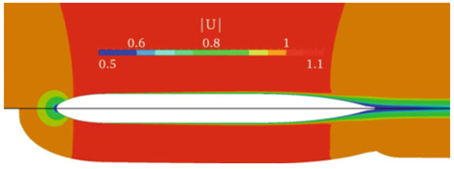
\includegraphics[width=0.6\textwidth]{figures/ch1-Helmholtz-Edmund.png}
	\caption{二维潜体湍流速度场\cite{edmundVelocitydecompositionFormulationIncompressible2013}：全粘流方法(上)和耦合方法(下)对比}
	\label{fig:ch1-Helmholtz-Edmund}
\end{myfigure}

Zhang\cite{zhangMultimodelMethodSimulating2018}采用了类似Kim等人\cite{kimComplementaryRANSEquations2005}的方法对速度进行分解，%
并通过两相流Euler求解器求解势流部分。%
值得注意的是，流固耦合问题在势流域中也需要求解，并且绕射波、辐射波等由欧拉方程求解。%
势流解通过松弛区域单向传递至粘流域，在这点上该方法与区域分解方法有相似之处。%
在他们的研究中，对复杂海底地形下的二维波浪结构物作用问题进行了模拟，与全粘流方法和试验结果基本一致，并且计算耗时能够节省50\%甚至85\%。

由互补NS方程求得的互补项中所包含的粘性效应，如果在实际计算中不加以处理，其衰减并不快。同时，在耦合计算中所有的粘流离散点都需要赋予势流解，因此对计算成本的减小并不显著。而Edmund\cite{edmundVelocityDecompositionMethod2012,edmundImprovedViscousInviscid2011,%
edmundVelocitydecompositionFormulationIncompressible2013}的方法虽然对粘流域进行了截断，但需要进行迭代运算，%
因此相比于Kim等\cite{kimComplementaryRANSEquations2005}的方法计算量更大。%
此外，在面对如波浪破碎等复杂的两相流问题时，进行速度分解是有困难的，因此Helmholtz速度分解法暂时只被用于较为简单问题的势粘流耦合研究。%

船舶和海洋工程相比其他领域而言，自由液面的存在是其一大突出特点，并且对自由液面的模拟增加了数值计算成本。%
基于此，研究人员提出了SWENSE模型。SWENSE模型最初由Ferrant等人\cite{ferrantNewRANSEPotential2002,ferrantPotentialRANSEApproach2003}提出，%
其基本思想是将速度、压力和自由面高度等分解为入射项和其他剩余项，如\cref{fig:ch1-SWENSE-示意图}所示。其表达如下：
\begin{equation}
	\bm{u} = \bm{u}_{\rm{I}} + \bm{u}_{\rm{D}},\quad %
	\bm{p} = \bm{p}_{\rm{I}} + \bm{p}_{\rm{D}},\quad %
	\bm{\eta} = \bm{\eta}_{\rm{I}} + \bm{\eta}_{\rm{D}}
\end{equation}
并推导得到修正的NS方程：
\begin{equation}
	\frac{\partial \bm{u}_{\rm{D}}}{\partial t} +\left(\bm{u}\cdot\nabla\right)\bm{u}_{\rm{D}} %
	- \nu\nabla^2\bm{u}_{\rm{D}} + \frac{\nabla p_{\rm{D}}}{\rho} %
	= - \left(\bm{u}_{\rm{D}}\cdot\nabla\right)\bm{u}_{\rm{I}} + \nu\nabla^2\bm{u}_{\rm{I}}
\end{equation}
式中$\nu$为运动粘性系数。二维情况下，质量守恒方程和运动学、动力学自由面条件为：
\begin{subequations}
	\begin{gather}
	\nabla\cdot\bm{u} = 0 \\ % 
	\frac{\partial \eta_{\rm{D}}}{\partial t} %
	+ \left(\bm{u}_{\rm{D}}\cdot\bm{i}\right)\left(\nabla\eta_{\rm{I}}\cdot\bm{i}\right) %
	+ \left(\bm{u}\cdot\bm{i}\right)\left(\nabla\eta_{\rm{D}}\cdot\bm{i}\right) %
	= \bm{u}_{\rm{D}}\cdot\bm{j} \\ % 不编号
	p_{\rm{D}} = \rho\bm{g}\eta_{\rm{D}} + 2\rho\nu\left(\nabla\cdot\bm{n}\right)\left(\bm{u}\cdot\bm{n}\right) \\ %
	\left(\bm{n}\cdot\nabla\right)\left(\bm{u}\cdot\bm{\tau}\right) %
	+ \left(\bm{\tau}\cdot\nabla\right)\left(\bm{u}\cdot\bm{n}\right) = 0 %
	\end{gather}
\end{subequations}
以上这一组方程即为SWENSE方程组。%
式中：$\bm{i}$、$\bm{j}$分别为水平和竖直方向的方向向量，$\bm{\tau}$和$\bm{n}$分别为自由液面处的切向和法向。%
SWENSE方程求解过程中，入射项由势流方法求解给出，而剩余项由SWENSE粘流求解器获得。%
在求解过程中，每一时间步内先由势流方法求解给出入射波，然后粘流求解器根据入射波求解辐射、绕射和粘性流动等问题。%
这是一种基于方程分解的单向耦合，粘流模型对势流没有反馈。
\begin{myfigure}
	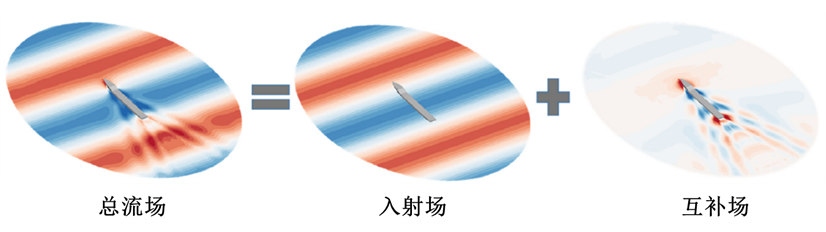
\includegraphics[width=0.8\textwidth]{figures/ch1-SWENSE-示意图.png}
	\caption{SWENSE模型示意图\cite{yuNumericalStudyWavestructure2022a}}
	\label{fig:ch1-SWENSE-示意图}
\end{myfigure}

Luquet等人\cite{luquetApplicationSWENSEMethod2007,luquetSimulationTLPWaves2007}%
和Alessandrini等人\cite{alessandriniNumericalSimulationShip2008}通过HOS方法给出入射波，%
对Wigley船在规则波中的二自由度运动以及固定半潜式平台在聚焦波中的载荷响应进行了全尺度模拟。%
Wigley船的垂荡和纵摇运动以及平台的载荷计算结果均与试验一致。%
Monroy等人\cite{monroyRANSSimulationsShip2009}使用该方法计算了重吊船在规则波和不规则波迎浪工况下的垂荡和纵摇响应，%
并进行了模型试验，其结果进一步验证了此数值方法的准确性。

早期的SWENSE模型未采用自由面捕捉技术，在解决自由面大变形、波浪破碎等复杂的两相流问题上较为困难。%
Reliquet等人\cite{reliquetSimulationWaveBodyInteraction2013,reliquetSimulationsDelft3722019}采用交错网格布置，配合LSM方法实现了两相流求解。%
采用该方法对静水和迎浪中船舶的模拟结果\cite{reliquetSimulationWaveBodyInteraction2013}与试验结果对比良好，%
如\cref{fig:ch1-SWENSE-Reliquet}所示。%
对不同傅汝德数下的双体船进行耐波性计算\cite{reliquetSimulationsDelft3722019}，其结果与全粘流方法以及试验结果吻合较好。%
进一步地，Vukčević\cite{vukcevicNumericalModellingCoupled2016}针对扰动波反射问题，在SWENSE求解器中添加了隐式松弛区域。%
类似地，他们的研究中也采用了LSM方法对自由面进行捕捉，模拟了二维数值水池和竖直圆柱的高阶波浪力。%
其数值结果与试验和文献结果吻合良好，并对计算中的波浪条件、离散条件等进行了分析。%
Gatin等人\cite{gatinFrameworkEfficientIrregular2017}采用Vukčević\cite{vukcevicNumericalModellingCoupled2016}的方法%
模拟了三维实尺度集装箱船遭遇极端波浪。%
在此工况下，船体出现了大幅横荡和横摇运动，并且捕捉到了上浪现象。%
除了LSM方法以外，Li等人\cite{liCalculationHighorderWave2017,liProgressCouplingPotential2018}将VOF方法引入SWENSE模型以实现两相流求解。%
通过对二维数值水池以及规则波中竖直圆柱的计算，验证了该方法的有效性和准确性，如\cref{fig:ch1-SWENSE-Li}所示。%
此外，Li等人\cite{liSpectralWaveExplicit2021}还模拟了规则波、不规则波工况下的固定CALM浮标模型，%
与全粘流方法和试验结果对比显示，在相同网格数下耦合方法精度好于全粘流方法，而在相同精度要求下其计算效率也高于后者。%
\begin{myfigure}
	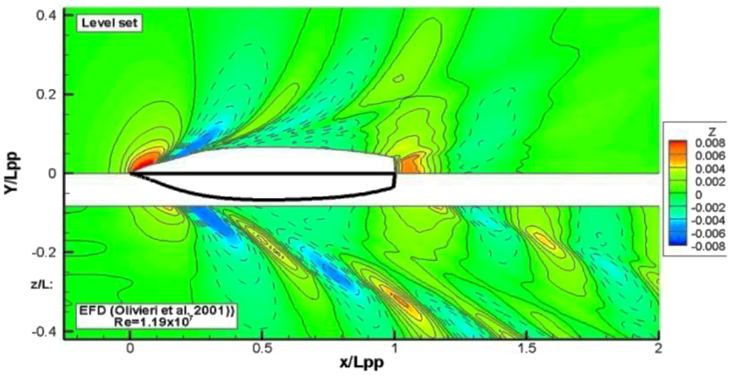
\includegraphics[width=0.6\textwidth]{figures/ch1-SWENSE-Reliquet.png}
	\caption{船体近场自由面高\cite{reliquetSimulationWaveBodyInteraction2013}：耦合方法(上半)与试验结果(下半)对比}
	\label{fig:ch1-SWENSE-Reliquet}
\end{myfigure}
\begin{myfigure}
	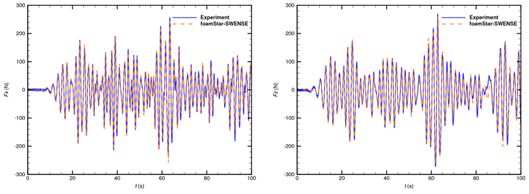
\includegraphics[width=0.8\textwidth]{figures/ch1-SWENSE-Li.png}
	\caption{CALM浮标波浪载荷\cite{liCalculationHighorderWave2017}：水平波浪力(左)和竖直波浪力(右)，耦合方法与试验结果对比}
	\label{fig:ch1-SWENSE-Li}
\end{myfigure}

SWENSE模型是目前较为成熟的势粘流耦合方程分解方法。%
由于SWENSE边界无需施加入射波条件，因此能够有效地降低方程组边界条件的复杂度，在保证精度的前提下提高计算速度。%
并且经过不断发展，该方法能够解决的问题类型也越来越丰富。%
但是SWENSE求解器的开发和优化难度较大，并且面对不合适求解的问题时修改的灵活性较差。

方程分解方法的研究进展总结如\cref{tab:ch1-FD-progress}所示。%
方程分解方法从流动控制方程中解耦出势流部分，采用势流方法对其独立求解，再将势流部分代入互补NS方程的求解以实现耦合。%
Helmholtz速度分解方法将流动分解为势流项和剩余项，因此辐射、绕射等问题一般由势流求解，而粘性、湍流等由互补NS方程求解。%
而SWENSE模型将流动分解为入射项和剩余项，其中入射项通过势流求解给出，因此辐射、绕射以及粘性和湍流等问题均由SWENSE求解器解得。%
\begin{mylongtable}
	{M{1.8cm} M{4.5cm} M{2cm} M{7.5cm}}
	{方程分解方法研究进展}
	{tab:ch1-FD-progress}
	{\toprule
		{分解模型} & {研究人员} & {自由面技术} & {应用问题} \\
		\midrule
	}
	{\multicolumn{4}{c}{\cref{tab:ch1-FD-progress} 方程分解方法研究进展(续表)} \\
		\toprule
		{分解模型} & {研究人员} & {自由面技术} & {应用问题} \\
		\midrule
	}
	{\bottomrule}
	{\bottomrule}
	& {Kim等\cite{kimComplementaryRANSEquations2005} (2005)} & {——} & {平板流、方形管道流、机翼绕流 (2D)} \\
	& {Hafez等\cite{hamiltonViscousInviscidMatching2011} (2007)} & {——} & {机翼绕流 (2D)} \\
	\multirow{2}{1.8cm}{\centering Helmoholtz速度分解} %
	& {Edmund等\cite{edmundVelocitydecompositionFormulationIncompressible2013} (2013)} & {——} & {二维翼型和圆柱绕流、潜体湍流 (2D、3D)} \\
	& {Rosemurgy等\cite{rosemurgyVelocityDecompositionApproach2012} (2012)} & {——} & {流过池底凸起结构的定常自由面流 (2D)} \\
	& {Chen等\cite{chenVelocityDecompositionApproach2015} (2015)} & {——} & {有限长平板层流、Wigley船湍流 (3D)} \\
	& {Zhang\cite{zhangMultimodelMethodSimulating2018} (2018)} & {VOF} & {复杂海底地形波浪结构物作用 (2D)} \\
	\hline
	& {Ferrant\cite{ferrantNewRANSEPotential2002,ferrantPotentialRANSEApproach2003} (2003)} & {——} & {规则波与固定方形潜体作用 (2D)} \\
	& \makecell{Luquet等\cite{luquetApplicationSWENSEMethod2007,luquetSimulationTLPWaves2007} (2007) \\ %
	Alessandrini等\cite{alessandriniNumericalSimulationShip2008}(2008)} & {——} & {Wigley船二自由度运动、聚焦波与固定半潜式平台作用 (3D)} \\
	& {Gentaz\cite{gentazNumericalSimulation3D2008} (2008)} & {——} & {波浪中的竖直圆柱 (3D)} \\
	& {Monroy等\cite{monroyRANSSimulationsShip2009} (2009)} & {——} & {重吊船在波浪中的二自由度响应 (3D)} \\
	\multirow{2}{1.8cm}{\centering SWENSE模型} %
	& {Reliquet等\cite{reliquetSimulationWaveBodyInteraction2013} (2013)} & {LSM} & {静水和迎浪中的船舶 (3D)} \\
	& {Reliquet等\cite{reliquetSimulationsDelft3722019} (2019)} & {LSM} & {不同傅汝德数下双体船的耐波性 (3D)} \\
	& {Vukčević等\cite{vukcevicNumericalModellingCoupled2016} (2016)} & {LSM} & {数值水池、竖直圆柱高阶波浪力 (2D、3D)} \\
	& {Gatin等人\cite{gatinFrameworkEfficientIrregular2017} (2017)} & {LSM} & {实尺度集装箱船遭遇极端波浪 (3D)} \\
	& {Li等\cite{liCalculationHighorderWave2017,liProgressCouplingPotential2018,liSpectralWaveExplicit2021} (2021)} %
	& {VOF} & {二维数值水池、规则波中的竖直圆柱、不同工况下的固定CALM浮标模型 (2D、3D)} \\
	& {Aliyar\cite{aliyarExtremeWaveInteraction2022} (2022)} & {VOF} & {圆柱波浪爬升、浮式风机波固耦合 (3D)} \\
	& {Yu等\cite{yuNumericalStudyWavestructure2022a} (2022)} & {LSM} & {有/无航速典型船舶在波浪中的动力响应 (3D)} \\
\end{mylongtable}

方程分解方法对船舶耐波性、波浪力计算等问题的解决比较成熟，%
在保持精度的前提下能够有效提高计算效率，甚至在同等计算资源条件下能够提高求解精度。%
虽然方程分解方法在两相流问题的解决上已经有很大进步，但是面对自由面大变形甚至波浪破碎等复杂问题时求解仍然困难。

\subsection{
  \texorpdfstring{本文研究内容及特点} % 正文和目录中显示的标题
  {\thesubsection 本文研究内容及特点} % 书签页中显示的标题
}
\label{ssec:本文研究内容及特点}

综上所述，恶劣海况下波浪与浮式平台强非线性作用这一多尺度问题的CFD方法数值模拟仍具有一些缺陷。%
第一，CFD方法在模拟大尺度极端波浪演化时具有严重的数值耗散和色散；%
第二，CFD方法在同时模拟大尺度波浪演化、主尺度平台运动以及小尺度砰击作用这一多尺度问题时，对计算资源的需求十分巨大并且是工程上难以接受的；%
第三，传统有网格CFD方法在模拟砰击这一类自由液面大变形问题时，需要在自由液面处布置大量精细网格以准确捕捉液面变化，这会带来更严重的计算消耗。%

因此本文尝试探索一种基于无网格CFD方法的势粘流耦合模型，将浮式平台遭受波浪强非线性作用这一多尺度问题进行分解并实现多模型耦合求解，%
以实现在保证计算精度的前提下尽量减少计算资源消耗。%
目前势粘流耦合方法研究主要集中于船舶耐波性操纵性、数值水池造波等问题，而针对波浪与结构物强非线性相互作用问题的研究较少。%
并且大多数势粘流耦合研究中所采用的CFD方法为有网格方法，而基于无网格CFD方法的势粘流耦合研究相对较少，耦合模型的计算精度和效率仍待提升。%

本文将采用区域分解方法进行基于无网格CFD方法的势粘流耦合模型开发，主要有以下几点原因：%
(1)区域分解方法和方程分解方法对自由液面不发生大变形的问题进行模拟时，二者的计算精度和效率相近\cite{robauxAssessmentOnewayCoupling2022}，%
但区域分解方法不需要修改NS控制方程，其开发和优化相对更为容易；%
(2)方程分解方法对于自由液面发生大变形、翻卷甚至破碎等问题的模拟较为复杂，对自由液面处的处理比较困难；%
(3)本文所采用的无网格CFD方法目前还不适合采用方程分解方法进行势粘流耦合。%

基于区域分解方法，波浪与浮式平台强非线性作用这一多尺度问题可以分解为大尺度波浪演化、主尺度平台运动和小尺度强非线性作用。%
在势粘流耦合模型中，大尺度波浪演化通过势流方法求解，而主尺度平台运动和小尺度砰击作用通过无网格CFD方法求解。%
这样一来既能够提高波浪模拟的质量，又能够有效地降低计算资源消耗，从而提高数值模拟的准确性和效率。%
本文将结合势流方法能够快速准确地模拟波浪的优势以及CFD方法能够模拟强非线性自由液面运动问题的能力，%
初步探索面向波浪与浮式平台强非线性作用问题的势粘流耦合方法，并在二维上实现数值算法开发。本文的主要工作内容如下：

(1)	基于高阶谱开源求解器HOS-NWT与改进的光滑粒子流体动力学$\delta^+$-SPH模型，构建HOS-SPH势粘流单向耦合模型，%
以实现通过HOS方法为SPH方法提供入射波边界条件，从而提高波浪模拟质量和计算效率；

(2)	基于有限水深二维时域Rankine源边界元法，在HOS-SPH势粘流单向耦合模型的基础上进行HOS-SPH-BEM势粘流多模型耦合算法开发，%
以实现势粘流间流场信息的双向传递，从而进一步提高数值计算精度；

(3)	对势粘流耦合算法进行验证和测试，主要考察对计算精度和效率的提高。

本文框架如\cref{fig:ch1-论文框架图}所示：
\begin{myfigure}
	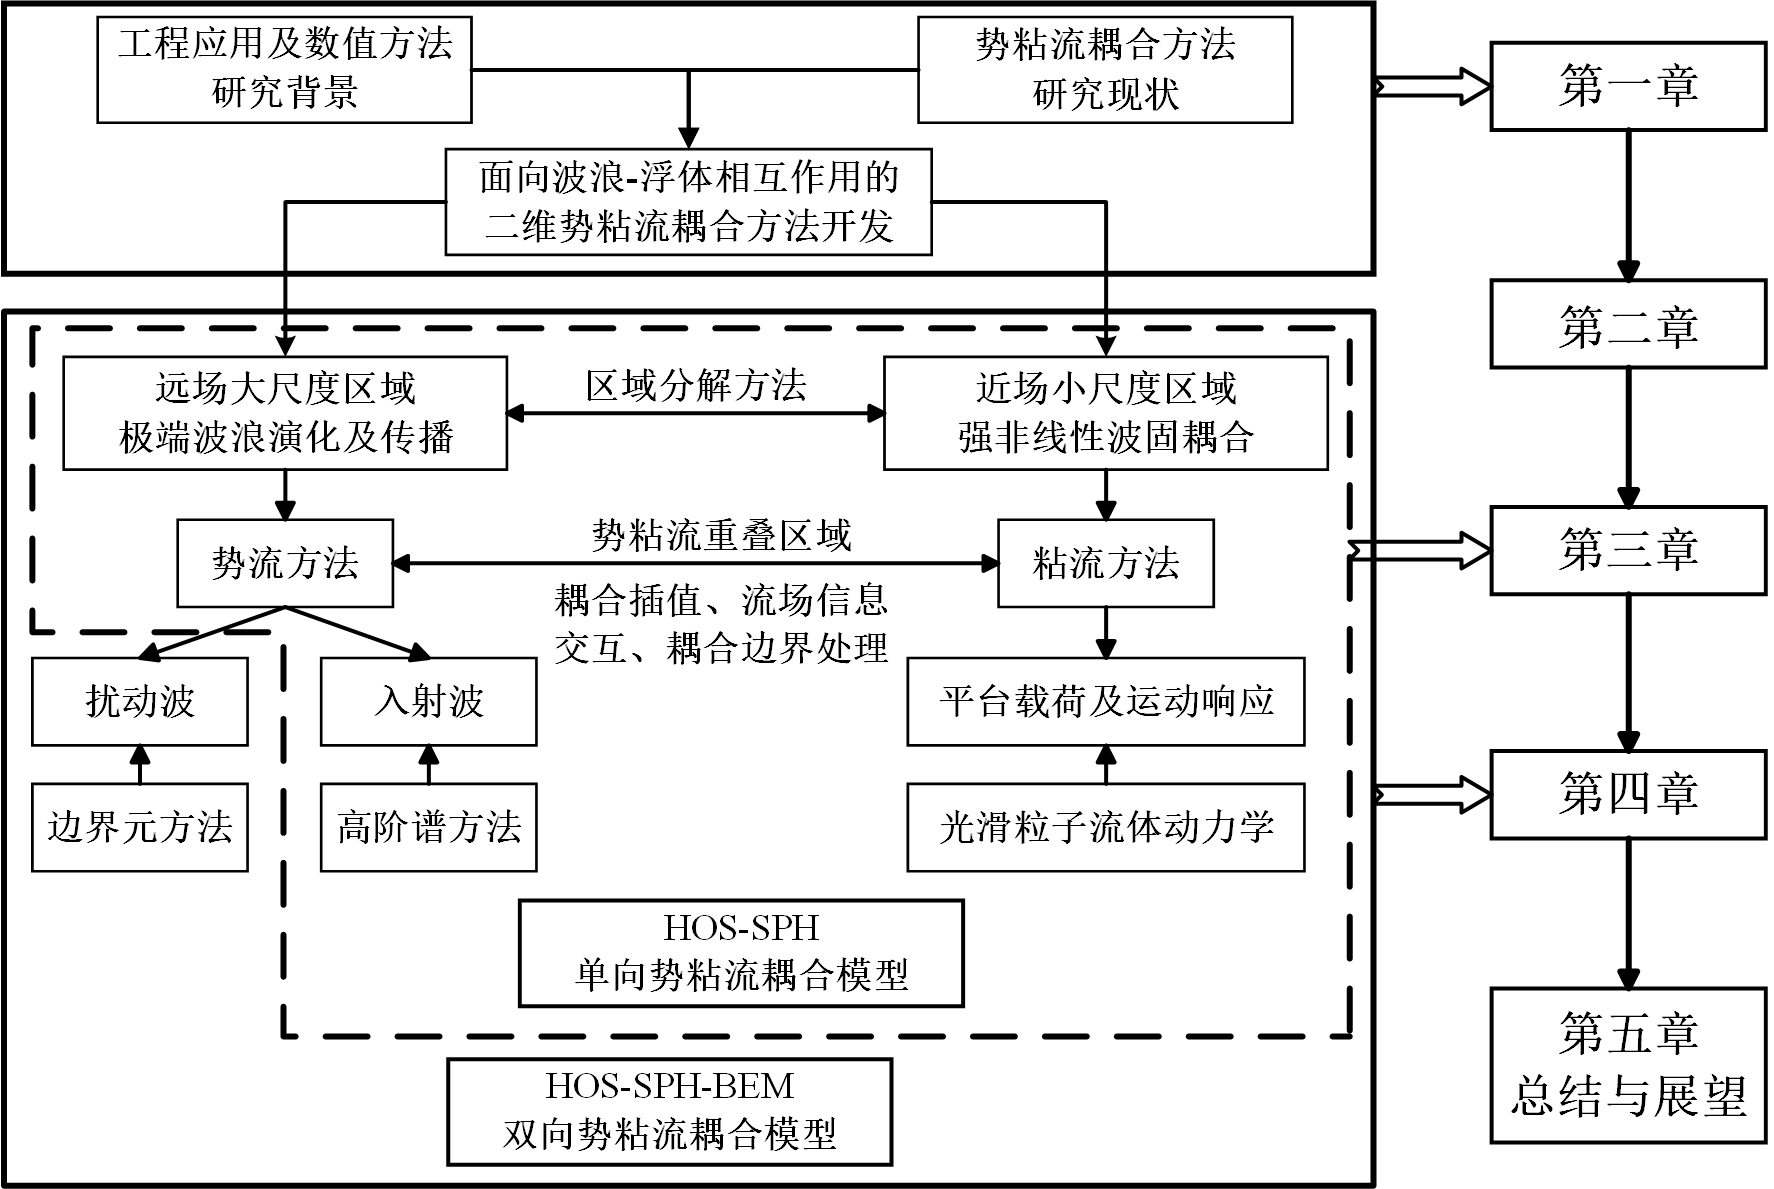
\includegraphics[width=0.99\textwidth]{figures/ch1-论文框架图.png}
	\caption{论文框架图}
	\label{fig:ch1-论文框架图}
\end{myfigure}

本文共分为五个章节，具体安排如下：%
第1章介绍选题背景与研究意义和势粘流耦合方法研究现状；%
第2章介绍所使用的数值方法和求解器，并通过数值波浪模拟对它们进行验证；%
第3章在HOS方法和SPH方法的基础上构建HOS-SPH势粘流单向耦合模型，并通过数值算例对HOS-SPH单向耦合方法进行验证和分析；%
第4章建立基于BEM方法和SPH方法的SPH-BEM势粘流双向耦合方法，并实现基于该方法的数值消波。%
而后在HOS-SPH单向耦合方法和SPH-BEM双向耦合方法的基础上进一步构建HOS-SPH-BEM势粘流多模型耦合方法，并对其进行验证；%
最后对全文的工作进行总结和展望。